\subsection{REAL-VALUED FUNCTIONS DEFINED ON A FILTERED SET}

PROPOSITION 1. Let \(f\) and \(g\) be two real-valued functions defined on a set \(\mathbf{X}\) filtered by a filter \(\mathfrak{F}\) . If \(\lim_{\mathfrak{F}} f\) and \(\lim_{\mathfrak{F}} g\) exist, and if, for each subset \(\mathbf{A} \in \mathfrak{F}\) , there exists \(x \in \mathbf{A}\) such that \(f(x) \leqslant g(x)\) , then we have \(\lim_{\mathfrak{F}} f \leqslant \lim_{\mathfrak{F}} g\) .

To prove this result we shall prove the following equivalent statement:

PROPOSITION 2. Let \(f\) and \(g\) be two real-valued functions defined on a set \(X\) filtered by a filter \(\mathfrak{F}\) . If \(\lim_{\mathfrak{F}} f\) and \(\lim_{\mathfrak{F}} g\) exist, and if \(\lim_{\mathfrak{F}} f > \lim_{\mathfrak{F}} g\) , then there is a set \(A \in \mathfrak{F}\) such that \(f(x) > g(x)\) for all \(x \in A\) .

Let \(a = \lim_{\mathfrak{F}} f\) , let \(b = \lim_{\mathfrak{F}} g\) and let \(c\) be such that \(b < c < a\) . The interval \(]c, +\infty]\) of \(\overline{\mathbf{R}}\) (resp. \([-\infty, c[)\) is a neighbourhood of \(a\) (resp. \(b\) ); hence there is a set \(M \in \mathfrak{F}\) (resp. a set \(N \in \mathfrak{F}\) ) such that \(f(x) > c\) for all \(x \in M\) {[}resp. \(g(x) < c\) for all \(x \in N\) {]}. The set \(A = M \cap N\) belongs to \(\mathfrak{F}\) , and we have \(f(x) > c > g(x)\) for all \(x \in A\) .

As a particular case of Proposition 1 we have the following theorem:

THEOREM 1 (Principle of extension of inequalities). Let \(f\) and \(g\) be two real-valued functions, defined on a set \(\mathbf{X}\) filtered by a filter \(\mathfrak{F}\) . If \(\lim_{\mathfrak{F}} f\) and \(\lim_{\mathfrak{F}} g\) exist, and if \(f \leqslant g\) , then \(\lim_{\mathfrak{F}} f \leqslant \lim_{\mathfrak{F}} g\) .

\pandocbounded{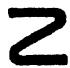
\includegraphics[keepaspectratio]{images/part002_67e89114.jpg}}

Remark. If in particular we have \(f(x) < g(x)\) for all \(x \in X\) (or only for all points of a set of the filter \(\overline{\mathbf{R}}\) ) we can infer, by Theorem 1, that \(\lim_{\mathfrak{F}} f \leqslant \lim_{\mathfrak{F}} g\) ; but we cannot infer the strong inequality \(\lim_{\mathfrak{F}} f < \lim_{\mathfrak{F}} g\) . For example, if we take \(X\) to be the set \(N\) of natural numbers, filtered by the Fréchet filter, and if \(f(n) = 0\) and \(g(n) = 1/n\) , then \(f(n) < g(n)\) for all \(n\) , but \(\lim_{n \to \infty} f(n) = \lim_{n \to \infty} f(n) = 0\) . Thus we lose strictness when we pass to the limit in a strict inequality.

THEOREM 2 (Theorem of the monotone limit). Let X be an ordered set and let A be a directed subset of X (*). Every monotonic real-valued function f defined on A has a limit with respect to A (Chapter I, § 7, no. 3); if f is increasing (resp. decreasing), this limit is equal to the least upper bound (resp. greatest lower bound) of the set \(f(A) \subset \overline{\mathbf{R}}\) .

Suppose for example that \(f\) is increasing, and let \(a = \sup f(A)\) . If \(a = -\infty\) , the theorem is trivial. If \(a > -\infty\) , then for each \(b < a\) there exists \(x \in A\) such that \(b < f(x) \leqslant a\) ; hence, if \(S_x\) is the section of \(A\) relative to \(x\) (i.e.~the set of all \(y \geqslant x\) , cf.~Chapter I, § 6, no. 3), \(f(S_x)\) is contained in the neighbourhood \(]b, +\infty]\) of \(a\) , and the theorem follows. The proof is analogous if \(f\) is decreasing.

COROLLARY. An increasing (resp. decreasing) real-valued function, defined on a directed subset A of an ordered set X, has a finite limit with respect to A if and only if it is bounded above (resp. bounded below) in A.

If we apply Theorem 2 to the case where \(\mathbf{A} = \mathbf{X} = \mathbf{N}\) (ordered by the relation \(\leqslant\) ), we have the following proposition:

PROPOSITION 3. Every monotonic sequence of real numbers has a limit in R. In particular, every increasing (resp. decreasing) sequence of finite numbers converges to a finite real number if it is bounded above (resp. bounded below) and to +∞ (resp. -∞) otherwise. For example, the sequence of positive integers converges to +∞.

This fact is the origin of the notation \(\lim_{n\to \infty}u_n\) to denote the limit of a sequence (Chapter I, § 7, no. 3).

Likewise, every strictly increasing sequence of integers \((p_n)\) converges to \(+\infty\) ; for we see by induction that \(p_n \geqslant p_0 + n\) for all \(n\) .

\subsection{LIMITS ON THE RIGHT AND ON THE LEFT OF A FUNCTION OF A REAL VARIABLE}

Let A be a non-empty subset of \(\overline{R}\) and let \(a \neq -\infty\) be a point of \(\overline{R}\) lying in the closure of the set \(B = A \cap [-\infty, a[\) . The set B is directed with respect to the relation \(\leqslant\) , and its section filter F is the same as the trace on B of the neighbourhood filter of a in \(\overline{R}\) .

DEFINITION 2. Let \(f\) be a function defined on a non-empty subset \(A\) of \(\overline{\mathbf{R}}\) , with values in a topological space \(X\) . A limit of \(f\) with respect to the filter \(\mathfrak{F}\) , if it exists, is called a limit of \(f\) on the left at the point \(a\) , relative to \(A\) , and is denoted by

\(\lim_{x \to a, x < a, x \in \mathbf{A}} f(x), \text{ or } f(a - ), \text{ if } \mathbf{X} \text{ is Hausdorff.}\)

Likewise, if \(a\) is in the closure of the set \(A \cap ]a, +\infty]\) , we define a limit on the right (if it exists) of \(f\) at the point \(a\) , and denote it by \(\lim_{x \to a, x > a, x \in A} f(x)\) , or \(f(a+)\) , if \(X\) is Hausdorff.

The following proposition is an immediate consequence of Theorem 2:

PROPOSITION 4. Let A be a subset of \(\overline{\mathbf{R}}\) and let \(a \neq -\infty\) be a point in the closure of the intersection \(\mathbf{A} \cap [-\infty, a[\) . If \(f\) is a monotonic real-valued function defined on A, then \(f\) has a limit \(f(a - )\) on the left at \(a\) , relative to A.

\subsection{BOUNDS OF A REAL-VALUED FUNCTION}

DEFINITION 3. Let \(f\) be a real-valued function defined on a set \(\mathbf{X}\) , and let \(\mathbf{A}\) be a non-empty subset of \(\mathbf{X}\) . Then the least upper bound (resp. greatest lower bound) of the set \(f(\mathbf{A})\) in \(\overline{\mathbf{R}}\) is called the least upper bound (resp. greatest lower bound) of \(f\) in \(\mathbf{A}\) , and is denoted by \(\sup_{x\in \mathbf{A}}f(x)\left[\text{resp. } \inf_{x\in \mathbf{A}} f(x)\right]\) .

In particular, if A is a non-empty subset of \(\overline{R}\) , then

\[
\sup \mathrm{A} = \sup _ {x \in \mathrm{A}} x.\tag{1}
\]

It is often more convenient to use the notation on the right-hand side to denote the least upper bound of A.

The number \(a = \sup_{x \in \mathbf{A}} f(x)\) is characterized by the following two properties:

\begin{enumerate}
\def\labelenumi{(\roman{enumi})}
\item
  For all \(x \in \mathbf{A}, f(x) \leqslant a\) .
\item
  For every \(b < a\) , there exists \(x \in \mathbf{A}\) such that \(b < f(x) \leqslant a\) .
\end{enumerate}

The numbers \(\sup_{x\in\mathbf{A}}f(x)\) and \(\inf_{x\in\mathbf{A}}f(x)\) belong to the closure of \(f(\mathbf{A})\) in \(\overline{\mathbf{R}}\) . We have \(\inf_{x\in\mathbf{A}}f(x)\leqslant\sup_{x\in\mathbf{A}}f(x)\) ; and these two numbers are equal if and only if \(f\) is constant on \(\mathbf{A}\) .

A real-valued function, defined on a set X, is bounded above (resp. bounded below) in a non-empty subset A of X if and only if \(\sup_{x\in\mathbf{A}}f(x)<+\infty\) {[}resp. \(\inf_{x\in\mathbf{A}}f(x)>-\infty\) {]}. f is bounded in A if and only if \(|f|\) is bounded above in A, hence if and only if \(\sup_{x\in\mathbf{A}}|f(x)|<+\infty\) .

We have

\[
\inf _ {x \in \mathbf {A}} f (x) = - \sup _ {x \in \mathbf {A}} (- f (x)).\tag{2}
\]

This relation reduces all properties of the greatest lower bound to those of the least upper bound; hence in general we shall speak only of the latter.

PROPOSITION 5. Let \(f\) be a real-valued function defined on a set \(\mathbf{X}\) . On the set \(\mathfrak{F}(\mathbf{X})\) of all finite subsets of \(\mathbf{X}\) , directed with respect to the relation \(\subset\) , the real-valued function \(\mathbf{H} \to \sup_{x \in \mathbf{H}} f(x)\) is increasing, the real-valued function \(\mathbf{H} \to \inf_{x \in \mathbf{H}} f(x)\) is decreasing, and we have

\[
\left\{ \begin{array}{l} \sup _ {x \in \mathbf {A}} f (x) = \lim _ {\mathbf {H} \in \mathfrak {F} (\mathbf {X})} (\sup _ {x \in \mathbf {H}} f (x)), \\ \inf _ {x \in \mathbf {A}} f (x) = \lim _ {\mathbf {H} \in \mathfrak {F} (\mathbf {X})} (\inf _ {x \in \mathbf {H}} f (x)). \end{array} \right.\tag{3}
\]

Let \(\varphi(\mathbf{H}) = \sup_{x \in \mathbf{H}} f(x)\) . Clearly \(\varphi\) is increasing, and therefore has a limit \(a\) (no. 2, Theorem 2); and since \(\varphi(\mathbf{H}) \leqslant \sup_{x \in \mathbf{A}} f(x)\) for all H, we have \(a \leqslant \sup_{x \in \mathbf{A}} f(x)\) (no. 2, Theorem 1). If we had \(a < \sup_{x \in \mathbf{A}} f(x)\) , then there would exist \(x_0 \in \mathbf{X}\) such that \(a < f(x_0)\) ; but this is a contradiction since \(\varphi(\mathbf{H}) \geqslant f(x_0)\) whenever \(x_0 \in \mathbf{H}\) .

In particular, by (1), if A is any non-empty subset of \(\overline{R}\) , we have

\[
\sup \mathrm{A} = \lim _ {\mathrm{H} \in \mathfrak {F} (\mathrm{A})} (\sup _ {x \in \mathrm{H}} x).\tag{4}
\]

PROPOSITION 6. Let \(f\) and \(g\) be two real-valued functions defined on \(\mathbf{X}\) . If \(f(x) \leqslant g(x)\) at every point \(x\) of a non-empty subset \(A\) of \(\mathbf{X}\) , then we have

\[
\left\{ \begin{array}{l} \sup _ {x \in \mathbf {A}} f (x) \leqslant \sup _ {x \in \mathbf {A}} g (x), \\ \inf _ {x \in \mathbf {A}} f (x) \leqslant \inf _ {x \in \mathbf {A}} g (x). \end{array} \right.\tag{5}
\]

PROPOSITION 7. Let \(f\) be a real-valued function defined on \(\mathbf{X}\) . If \(\mathbf{A}\) and \(\mathbf{B}\) are two non-empty subsets of \(\mathbf{X}\) such that \(\mathbf{A} \subset \mathbf{B}\) , then

\[
\sup _ {x \in \mathbf {A}} f (x) \leqslant \sup _ {x \in \mathbf {B}} f (x).\tag{6}
\]

PROPOSITION 8. Let \(f\) be a real-valued function defined on \(\mathbf{X}\) , and let \((\mathbf{A}_t)_{t \in I}\) be a non-empty family of non-empty subsets of \(\mathbf{X}\) ; then

\[
\sup_{x\in \bigcup_{t\in \mathbf{I}}\mathbf{A}_{t}}f(x) = \sup_{t\in \mathbf{I}}(\sup_{x\in \mathbf{A}_{t}}f(x)).\tag{7}
\]

Let \(f\) be a real-valued function defined on a product set \(\mathbf{X}_1 \times \mathbf{X}_2\) . If \(\mathbf{A}_2\) is a non-empty subset of \(\mathbf{X}_2\) we shall denote by \(\sup_{x_2 \in \mathbf{A}_2} f(x_1, x_2)\) the least upper bound in \(\mathbf{A}_2\) of the real-valued function \(x_2 \to f(x_1, x_2)\) defined on \(\mathbf{X}_2\) . From Proposition 8 we deduce in particular:

PROPOSITION 9. Let \(f\) be a real-valued function defined on a product set \(\mathbf{X}_1 \times \mathbf{X}_2\) . If \(\mathbf{A}_1, \mathbf{A}_2\) are any non-empty subsets of \(\mathbf{X}_1, \mathbf{X}_2\) respectively, then

\[
\sup _ {(x _ {1}, x _ {2}) \in \mathbf {A} _ {1} \times \mathbf {A} _ {2}} f (x _ {1}, x _ {2}) = \sup _ {x _ {1} \in \mathbf {A} _ {1}} (\sup _ {x _ {2} \in \mathbf {A} _ {2}} f (x _ {1}, x _ {2})) = \sup _ {x _ {2} \in \mathbf {A} _ {2}} (\sup _ {x _ {1} \in \mathbf {A} _ {1}} f (x _ {1}, x _ {2})).\tag{8}
\]

\subsection{ENVELOPES OF A FAMILY OF REAL-VALUED FUNCTIONS}

DEFINITION 4. Let \((f_{t})_{t\in I}\) be a family of real-valued functions defined on a set X. The real-valued function on X whose value at each point \(x\in X\) is \(\sup_{t\in I}(f_t(x))\) {[}resp. inf \((f_t(x))]\) is called the upper (resp. lower) envelope of the family \((f_t)\) , and is denoted by \(\sup_{t\in I}f_{t}\) or \(\sup_{t}f_{t}\) (resp. inf \(f_{t}\) or inf \(f_{t}\) ).

The upper envelope of the family \((f_{t})\) is thus the least upper bound of this family in the lattice \(\overline{R}\) of real-valued functions defined on X, and this justifies the notation \(\sup f_{t}\) .

Furthermore, if we endow \(\overline{\mathbf{R}}^{\mathbf{X}}\) with the topology which is the product of the topologies of its factors (all identical with \(\overline{R}\) ), we have the following proposition:

PROPOSITION 10. In the product space \(\overline{\mathbf{R}}^{\mathbf{X}}\) the upper envelope \(\sup f_{t}\) of a family of real-valued functions \((f_{t})_{t\in I}\) is the limit, with respect to the directed set \(\mathfrak{F}(\mathbf{I})\) of finite subsets of \(\mathbf{I}\) , of the mapping \(\mathrm{H}\to \sup_{t\in \mathbf{H}}f_t\) {[}which maps each finite subset \(\mathrm{H}\) of \(\mathbf{I}\) to the upper envelope of the finite subfamily \((f_{t})_{t\in H}]\) .

This follows immediately from Proposition 5 of no. 4 and from Chapter I, § 7, no. 6, Corollary 1 to Proposition 10.

We may therefore write

\[
\sup _ {t \in I} f _ {t} = \lim _ {H \in \mathfrak {F} (I)} \left(\sup _ {t \in H} f _ {t}\right).\tag{9}
\]

DEFINITION 5. A family \((f_t)_{i\in I}\) of real-valued functions defined on a set \(\mathbf{X}\) is said to be uniformly bounded above (resp. uniformly bounded below) in \(\mathbf{X}\) , if there exists a finite number \(a\) such that \(f_{t}(x) \leqslant a\) {[}resp. \(f_{t}(x) \geqslant a\) {]} for all \(x \in X\) and all \(t \in I\) . The family \((f_{t})\) is said to be uniformly bounded in \(X\) if it is uniformly bounded above and below in \(X\) .

Thus \((f_{t})\) is uniformly bounded above in \(\mathbf{X}\) if and only if the upper envelope of this family is bounded above in \(\mathbf{X}\) . \((f_{t})\) is uniformly bounded in \(\mathbf{X}\) if and only if the upper envelope of the family \((|f_{t}|)\) is bounded above in \(\mathbf{X}\) {[}i.e.~if and only if there is a finite real number \(a \geqslant 0\) such that \(|f_{t}(x)| \leqslant a\) for all \(x \in \mathbf{X}\) and all \(t \in I\) {]}.

\subsection{UPPER LIMIT AND LOWER LIMIT OF A REAL-VALUED FUNCTION WITH RESPECT TO A FILTER}

Let \(f\) be a real-valued function defined on a set \(\mathbf{X}\) filtered by a filter \(\mathfrak{G}\) . \(\mathfrak{G}\) is a directed set with respect to the relation \(\supset\) (Chapter I, § 6). For each \(\mathbf{M} \in \mathfrak{G}\) consider the real number \(\sup_{x \in \mathbf{M}} f(x)\) : we have a function \(\mathbf{M} \to \sup_{x \in \mathbf{M}} f(x)\) of \(\mathfrak{G}\) into \(\overline{\mathbf{R}}\) , which is a decreasing function on \(\mathfrak{G}\) , by Proposition 7 of no. 4. Hence, by Theorem 2 of no. 2, it has a limit with respect to the directed set \(\mathfrak{G}\) .

DEFINITION 6. The limit of the real-valued function \(\mathbf{M} \to \sup_{x \in \mathbf{M}} f(x)\) with respect to the directed set \(\mathfrak{G}\) is called the upper limit of \(f\) with respect to the filter \(\mathfrak{G}\) , and is denoted by \(\lim \sup_{\mathfrak{G}} f\) , or by \(\lim \sup_{x, \mathfrak{G}} f(x)\) .

The lower limit of \(f\) with respect to the filter \(\mathfrak{G}\) is defined similarly, and is denoted by \(\liminf_{\mathfrak{G}} f\) or \(\liminf_{x, \mathfrak{G}} f(x)\) . Thus we have

\[
\left\{ \begin{array}{l} \lim \sup_{\mathfrak{G}} f = \lim_{\mathbf {M} \in \mathfrak {G}}(\sup_{x \in \mathbf {M}}f(x)), \\ \lim \inf_{\mathfrak{G}} f = \lim_{\mathbf {M} \in \mathfrak {G}}(\inf_{x \in \mathbf {M}}f(x)). \end{array} \right.\tag{10}
\]

Often the filter \(\mathfrak{G}\) is suppressed from the notation, and we write simply \(\lim \sup f\) or \(\lim \sup_x f(x)\) , or \(\lim \sup f(x)\) when there is no risk of confusion.

From formulae (10) and Theorem 1 we have

\[
\inf _ {x \in \mathbf {X}} f (x) \leqslant \lim \inf _ {\mathfrak {G}} f \leqslant \lim \sup _ {\mathfrak {G}} f \leqslant \sup _ {x \in \mathbf {X}} f (x).\tag{11}
\]

By Theorem 2 of no. 2 we may also write

\[
\left\{\lim \sup _ {\mathfrak {G}} f = \inf _ {\mathbf {M} \in \mathfrak {G}} (\sup _ {x \in \mathbf {M}} f (x)), \right.\tag{12}
\]

\[
\left\{\lim \inf _ {\mathfrak {G}} f = \sup _ {\mathbf {M} \in \mathfrak {G}} (\inf _ {x \in \mathbf {M}} f (x)). \right.
\]

Also we may replace the filter \(\mathfrak{G}\) , on the right-hand sides of formulae (10) and (12), by any base \(\mathfrak{B}\) of \(\mathfrak{G}\) .

From (2) and (10),

\[
\lim \inf _ {\mathfrak {G}} f = - \lim \sup _ {\mathfrak {G}} (- f)\tag{13}
\]

and therefore we need consider only the upper limit.

THEOREM 3. The upper limit of a real-valued function \(f\) with respect to a filter \(\mathfrak{G}\) is equal to the largest cluster value of \(f\) with respect to \(\mathfrak{G}\) .

Let \(b\) be a cluster point of \(f\) with respect to \(\mathfrak{G}\) . For each \(\mathbf{M} \in \mathfrak{G}\) , \(b\) lies in the closure of \(f(\mathbf{M})\) , hence \(b \leqslant \sup_{x \in \mathbf{M}} f(x)\) , and therefore, by (12), \(b \leqslant \limsup_{\mathfrak{G}} f = a\) .

On the other hand, let V be any open neighbourhood of a in \(\overline{R}\) . Then there exists a set \(M_{0}\) in G such that, for each \(M \in G\) contained in \(M_{0}\) , we have \(\sup_{x \in M} f(x) \in V\) ; since V is open it follows that \(f(M)\) meets V, and therefore a is a cluster point of f with respect to G, and the proof is complete.

COROLLARY 1. In order that \(\limsup_{\mathfrak{G}}f = \liminf_{\mathfrak{G}}f\) , it is necessary and sufficient that \(f\) has a limit with respect to the filter \(\mathfrak{G}\) , and then

\[
\lim _ {\mathfrak {G}} f = \lim \sup _ {\mathfrak {G}} f = \lim \inf _ {\mathfrak {G}} f.
\]

For since \(\overline{\mathbf{R}}\) is compact, the filter base \(f(\mathfrak{G})\) has a limit point if and only if it has only one cluster point (Chapter I, § 9, no. 1, Corollary to Theorem 1).

COROLLARY 2. If \(\mathfrak{H}\) is a filter finer than \(\mathfrak{G}\) , we have

\[
\lim \inf _ {\mathfrak {G}} f \leqslant \lim \inf _ {\mathfrak {H}} f \leqslant \lim \sup _ {\mathfrak {H}} f \leqslant \lim \sup _ {\mathfrak {G}} f.
\]

For every cluster point of \(f\) with respect to \(\mathfrak{H}\) is also a cluster point of \(f\) with respect to \(\mathfrak{G}\) (Chapter I, § 7, no. 3).

In particular, if \(\lim_{\mathfrak{H}}f\) exists, then

\[
\lim \inf _ {\mathfrak {G}} f \leqslant \lim _ {\mathfrak {H}} f \leqslant \lim \sup _ {\mathfrak {G}} f.
\]

COROLLARY 3. Let A be a set of the filter G, let \(\mathfrak{G}_{\mathbf{A}}\) be the filter induced on A by G, and let \(f_{\mathbf{A}}\) be the restriction of \(f\) to A; then

\[
\lim \sup _ {\mathfrak {G} _ {\mathbf {A}}} f _ {\mathbf {A}} = \lim \sup _ {\mathfrak {G}} f.
\]

For every cluster point of the filter base \(f(\mathfrak{G})\) is a cluster point of the filter base \(f_{\mathrm{A}}(\mathfrak{G}_{\mathrm{A}})\) , and conversely.

For this reason, if \(f\) is defined only on a subset \(A\) of \(X\) belonging to \(\mathfrak{G}\) , we shall often write \(\limsup_{\mathfrak{G}} f\) instead of \(\limsup_{\mathfrak{G}_{\mathbf{A}}} f_{\mathbf{A}}\) , by abuse of language.

PROPOSITION 11. Let \(f\) and \(g\) be two real-valued functions defined on a filtered set \(X\) . Then the relation \(f \leqslant g\) implies

\[
\left\{ \begin{array}{l} \lim \sup f \leqslant \lim \sup g, \\ \lim \inf f \leqslant \lim \inf g. \end{array} \right.\tag{14}
\]

This is an immediate consequence of the relations (12).

When X is a topological space and \(\mathfrak{G}\) is the neighbourhood filter of a point \(a\) of X, we write \(\limsup_{x\to a}f(x)\) {[}resp. \(\liminf_{x\to a}f(x)]\) in place of \(\limsup_{\mathfrak{G}}f\) {[}resp. \(\liminf_{\mathfrak{G}}f]\) ; clearly we have

\[
\liminf _ {x \to a} f (x) \leqslant f (a) \leqslant \limsup _ {x \to a} f (x).\tag{15}
\]

More generally, if X is a subspace of a topological space Y, and if G is the trace on X of the neighbourhood filter of a point \(a \in \overline{X}\) , we write \(\limsup_{x \to a, x \in X} f(x)\) {[}resp. \(\liminf_{x \to a, x \in X} f(x)\) {]} instead of \(\limsup_{\mathfrak{G}} f\) {[}resp. \(\liminf_{\mathfrak{G}} f\) {]}; \(\limsup_{x \to a, x \in X} f(x)\) is called the upper limit of \(f(x)\) as x tends to a while remaining in X. If X is the complement of \(\{a\}\) we write `` \(x \neq a\) '' in place of `` \(x \in X\) '' in these notations.

If \(\mathbf{A}\) is a subset of \(\mathbf{X}\) such that \(a \in \overline{\mathbf{A}}\) , then (Corollary 2 to Theorem 3)

\[
\liminf _ {x \to a, x \in \mathbf {X}} f (x) \leqslant \liminf _ {x \to a, x \in \mathbf {A}} f (x) \leqslant \limsup _ {x \to a, x \in \mathbf {A}} f (x) \leqslant \limsup _ {x \to a, x \in \mathbf {X}} f (x).
\]

If V is a neighbourhood of \(a\) in Y, we have (Corollary 3 to Theorem 3)

\[
\lim \sup _ {x \to a, x \in \mathbf {V} \cap \mathbf {X}} f (x) = \lim \sup _ {x \to a, x \in \mathbf {X}} f (x).
\]

Hence the notions of upper and lower limits at a point of a topological space are, like the notion of limit, of local character.

Finally, if \(\mathfrak{G}\) is the Fréchet filter on \(\mathbf{N}\) , the upper (resp. lower) limit, with respect to \(\mathfrak{G}\) , of the mapping \(n \to u_n\) of \(\mathbf{N}\) into \(\overline{\mathbf{R}}\) is denoted by \(\limsup_{n \to \infty} u_n\) (resp. \(\liminf_{n \to \infty} u_n\) ) and is called the upper (resp. lower) limit of the sequence of real numbers \(u_n\) .

The relation \(\limsup_{n\to \infty}u_n = a\in \mathbb{R}\) is therefore equivalent to the following: given any \(\varepsilon >0\) there exists an integer \(n_0\) such that, for each \(n\geqslant n_0\) we have \(u_{n}\leqslant a + \varepsilon\) , and for an infinity of values of \(n\) we have \(u_{n}\geqslant a - \varepsilon\) . The definition of the upper limit of a sequence may be translated similarly when its value is \(+\infty\) or \(-\infty\) .

Given a sequence \((f_n)\) of real-valued functions defined on a set \(\mathbf{X}\) , we denote by \(\limsup_{n\to \infty}f_n\) (resp. \(\liminf_{n\to \infty} f_n\) ) the real-valued function whose value at any point \(x\in \mathbf{X}\) is \(\limsup_{n\to \infty}f_n(x)\) {[}resp. \(\liminf_{n\to \infty} f_n(x)\) {]}. From (10) and (12) we deduce

\[
\left\{\begin{array}{l}\lim \sup _ {n \rightarrow \infty} f _ {n} = \inf _ {n \in \mathbb {N}} (\sup _ {m \geqslant n} f _ {m}) = \lim _ {n \rightarrow \infty} (\sup _ {m \geqslant n} f _ {m}),\\\lim \inf _ {n \rightarrow \infty} f _ {n} = \sup _ {n \in \mathbb {N}} (\inf _ {m \geqslant n} f _ {m}) = \lim _ {n \rightarrow \infty} (\inf _ {m \geqslant n} f _ {m}),\end{array}\right.\tag{16}
\]

the limits being taken in the product space \(\overline{\mathbf{R}}^{\mathbf{X}}\) . The sequence \((f_n)\) has a limit in \(\overline{\mathbf{R}}^{\mathbf{X}}\) if and only if \(\limsup_{n\to\infty}f_n=\liminf_{n\to\infty}f_n\) (Corollary 1 to Theorem 3, and Chapter I, § 7, no. 6, Corollary 1 to Proposition 10).

\subsection{ALGEBRAIC OPERATIONS ON REAL-VALUED FUNCTIONS}

Let \(f\) and \(g\) be two real-valued functions defined on a set \(\mathbf{X}\) ; if the sum \(f(x) + g(x)\) {[}resp. the product \(f(x)g(x)\) {]} is defined for all \(x \in \mathbf{X}\) , then we denote by \(f + g\) (resp. \(fg\) ) the real-valued function

\[
x \rightarrow f (x) + g (x) \quad [ \text { resp. } x \rightarrow f (x) g (x) ].
\]

Again, if \(1 / f(x)\) is defined for all \(x\in \mathbf{X}\) , then \(1 / f\) denotes the function \(x\to 1 / f(x)\) .

This last function is therefore defined provided \(f\) does not take the value \(0\) ; when \(f\) takes its values in the interval \([0, +\infty]\) (resp. in \([-\infty, 0]\) ) \(1/f(x)\) as everywhere defined by putting \(1/0 = +\infty\) (resp. \(1/0 = -\infty\) ); in this case the function \(1/f\) is defined.

Suppose that X is filtered by a filter \(\mathfrak{F}\) , and that \(\lim_{\mathfrak{F}} f\) and \(\lim_{\mathfrak{F}} g\) exist. If on the one hand the function \(f + g\) (resp. \(fg\) , \(1/g\) ) is defined, and if on the other hand the expression \(\lim_{\mathfrak{F}} f + \lim_{\mathfrak{F}} g\) (resp. \(\lim_{\mathfrak{F}} f\) . \(\lim_{\mathfrak{F}} g\) , \(1/\lim_{\mathfrak{F}} f\) ) has a sense, then \(\lim_{\mathfrak{F}} (f + g)\) {[}resp. \(\lim_{\mathfrak{F}} fg\) , \(\lim_{\mathfrak{F}} (1/f)\) {]} exists and is equal to this expression by reason of the continuity of the function \(x + y\) (resp. \(xy\) , \(1/x\) ) at points where it is defined.

PROPOSITION 12. Let \(f\) and \(g\) be two real-valued functions defined on a set \(\mathbf{X}\) , and let \(\mathbf{A}\) be a non-empty subset of \(\mathbf{X}\) .

\textit{(i) We have}

\begin{enumerate}
\def\labelenumi{(\arabic{enumi})}
\setcounter{enumi}{16}
\tightlist
\item
\end{enumerate}

\[
\sup _ {x \in \mathbf {A}} (f (x) + g (x)) \leqslant \sup _ {x \in \mathbf {A}} f (x) + \sup _ {x \in \mathbf {A}} g (x),\tag{17}
\]

\[
\sup _ {x \in \mathbf {A}} f (x) + \inf _ {x \in \mathbf {A}} g (x) \leqslant \sup _ {x \in \mathbf {A}} (f (x) + g (x)),\tag{18}
\]

whenever both sides of these inequalities are defined.

\begin{enumerate}
\def\labelenumi{(\roman{enumi})}
\setcounter{enumi}{1}
\tightlist
\item
  If \(f(x)\) and \(g(x)\) are \(\geqslant 0\) for each \(x \in \mathbf{A}\) , then
\end{enumerate}

\begin{enumerate}
\def\labelenumi{(\arabic{enumi})}
\setcounter{enumi}{18}
\tightlist
\item
\end{enumerate}

\[
\sup _ {x \in \mathbf {A}} (f (x) g (x)) \leqslant \sup _ {x \in \mathbf {A}} f (x) \sup _ {x \in \mathbf {A}} g (x),\tag{19}
\]

\[
\sup _ {x \in \mathbf {A}} f (x) \inf _ {x \in \mathbf {A}} g (x) \leqslant \sup _ {x \in \mathbf {A}} (f (x) g (x))\tag{20}
\]

whenever both sides of these inequalities are defined.

\begin{enumerate}
\def\labelenumi{(\roman{enumi})}
\setcounter{enumi}{2}
\tightlist
\item
  If \(f(x) \geqslant 0\) for all \(x \in \mathbf{A}\) , then
\end{enumerate}

\[
\sup _ {x \in \mathbf {A}} (1 / f (x)) = \inf _ {x \in \mathbf {A}} f (x)\tag{21}
\]

(putting \(1 / 0 = +\infty\) ).

Let \(\mathbf{H}\) be any finite subset of \(\mathbf{A}\) . If \(x_0\) is one of the points of \(\mathbf{H}\) where \(f + g\) takes its greatest value, then we have

\[
f (x _ {0}) + g (x _ {0}) \leqslant \sup _ {x \in \mathbf {H}} f (x) + \sup _ {x \in \mathbf {H}} g (x);
\]

on the other hand, if \(x_{1}\) is one of the points of \(H\) where \(f\) takes its greatest value, then

\[
f (x _ {1}) + g (x _ {1}) \geqslant \sup _ {x \in \mathbf {H}} f (x) + \inf _ {x \in \mathbf {H}} g (x);
\]

therefore

\[
\sup _ {x \in \mathbf {H}} f (x) + \inf _ {x \in \mathbf {H}} g (x) \leqslant \sup _ {x \in \mathbf {H}} (f (x) + g (x)) \leqslant \sup _ {x \in \mathbf {H}} f (x) + \sup _ {x \in \mathbf {H}} g (x).
\]

The inequalities (17) and (18) follow from this by applying Proposition 5 of no. 4 and Theorem 1 of no. 2. The proofs of the other inequalities are analogous.

COROLLARY 1. Let \(f\) be a real-valued function defined on \(\mathbf{X}\) , and let \(k\) be a real number. Then

\[
\sup _ {x \in \mathbf {A}} (f (x) + k) = k + \sup _ {x \in \mathbf {A}} f (x)\tag{22}
\]

whenever both sides are defined, and, if \(k \geqslant 0\) ,

\[
\sup _ {x \in \mathbf {A}} (k f (x)) = k. \sup _ {x \in \mathbf {A}} f (x)\tag{23}
\]

whenever both sides are defined.

COROLLARY 2. Let \(f_{1}\) and \(f_{2}\) be two real-valued functions defined on sets \(X_{1}, X_{2}\) respectively; then if \(A_{1}, A_{2}\) are any non-empty subsets of \(X_{1}, X_{2}\) respectively, we have

\[
\sup _ {(x _ {1}, x _ {2}) \in \mathbf {A} _ {1} \times \mathbf {A} _ {2}} (f _ {1} (x _ {1}) + f _ {2} (x _ {2})) = \sup _ {x _ {1} \in \mathbf {A} _ {1}} f _ {1} (x _ {1}) + \sup _ {x _ {2} \in \mathbf {A} _ {2}} f _ {2} (x _ {2})\tag{24}
\]

whenever both sides are defined; and if \(f_1, f_2\) are \(\geqslant 0\) in \(A_1, A_2\) respectively we have

\[
\sup _ {(x _ {1}, x _ {2}) \in \mathbf {A} _ {1} \times \mathbf {A} _ {2}} (f _ {1} (x _ {1}) f _ {2} (x _ {2})) = \sup _ {x _ {1} \in \mathbf {A} _ {1}} f _ {1} (x _ {1}) \sup _ {x _ {2} \in \mathbf {A} _ {2}} f _ {2} (x _ {2}),\tag{25}
\]

whenever both sides are defined.

This is an immediate consequence of the preceding corollary and Proposition 9 of no. 4.

In particular, if \(\mathbf{A}\) and \(\mathbf{B}\) are two subsets of \(\overline{\mathbf{R}}\) such that the set \(\mathbf{A} + \mathbf{B}\) of sums \(x + y\) ( \(x \in \mathbf{A}, y \in \mathbf{B}\) ) is defined, we have

\[
\sup (\mathbf {A} + \mathbf {B}) = \sup \mathbf {A} + \sup \mathbf {B}\tag{26}
\]

if the right-hand side is defined. Again, if A and B are two subsets of \([0, +\infty]\) , we have

\[
\sup \mathbf {A B} = \sup \mathbf {A}. \sup \mathbf {B}\tag{27}
\]

whenever both sides are defined.

PROPOSITION 13. Let \(f\) and \(g\) be two real-valued functions defined on a filtered set \(X\) .

\begin{enumerate}
\def\labelenumi{(\roman{enumi})}
\tightlist
\item
  We have
\end{enumerate}

\[
\lim \sup (f + g) \leqslant \lim \sup f + \lim \sup g, \tag {28}
\]

\begin{enumerate}
\def\labelenumi{(\arabic{enumi})}
\setcounter{enumi}{28}
\tightlist
\item
  \(\lim \sup f + \lim \inf g \leqslant \lim \sup (f + g)\)
\end{enumerate}

whenever both sides of these inequalities are defined.

\begin{enumerate}
\def\labelenumi{(\roman{enumi})}
\setcounter{enumi}{1}
\tightlist
\item
  If \(f\) and \(g\) are \(\geqslant 0\) on \(\mathbf{X}\) , we have
\end{enumerate}

\[
\lim \sup f g \leqslant (\lim \sup f) (\lim \sup g), \tag {30}
\]

\[
(\lim \sup f) (\lim \inf g) \leqslant \lim \sup f g \tag {31}
\]

whenever both sides of these inequalities are defined.

\begin{enumerate}
\def\labelenumi{(\roman{enumi})}
\setcounter{enumi}{2}
\tightlist
\item
  If \(f \geqslant 0\) on \(\mathbf{X}\) , then
\end{enumerate}

\[
\lim \sup (1 / f) = 1 / (\lim \inf f)\tag{32}
\]

(putting \(1 / 0 = +\infty\) ).

These relations are consequences of Proposition 12 and relations (10)

COROLLARY 1. Let \(f\) and \(g\) be two real-valued functions defined on a filtered set \(X\) . If \(\lim g\) exists, then

\[
\lim \sup (f + g) = \lim \sup f + \lim g \tag {33}
\]

whenever both sides are defined, and

\[
\lim \sup f g = (\lim \sup f) (\lim g) \tag {34}
\]

whenever both sides are defined and \(f\) and \(g\) are \(\geqslant 0\) .

COROLLARY 2. Let \(f\) and \(g\) be two real-valued functions defined on a filtered set X. If \(\lim f = +\infty\) and \(\lim \inf g > -\infty\) and \(f + g\) is defined, then \(\lim (f + g) = +\infty\) . If \(\lim f = +\infty\) and \(\lim \inf g > 0\) and \(fg\) is defined, then \(\lim fg = +\infty\) .

\section{CONTINUOUS AND SEMI-CONTINUOUS REAL-VALUED FUNCTIONS}

\subsection{CONTINUOUS REAL-VALUED FUNCTIONS}

Besides the general properties of continuous functions with values in an arbitrary topological space (Chapter I, § 2), continuous real-valued functions have the following two fundamental properties:

THEOREM 1 (Weierstrass). Let \(f\) be a continuous real-valued function defined on a non-empty quasi-compact space \(\mathbf{X}\) . Then there is at least one point \(a \in \mathbf{X}\) such that \(f(a) = \sup_{x \in \mathbf{X}} (f(x))\) , and at least one point \(b \in \mathbf{X}\) such that \(f(b) = \inf_{x \in \mathbf{X}} f(x)\) . For \(f(\mathbf{X})\) is compact (Chapter I, § 9, no. 4, Theorem 2) and therefore closed in \(\overline{\mathbf{R}}\) ; hence \(f(\mathbf{X})\) contains its bounds.

This theorem is often stated in the form that a continuous real-valued function on a non-empty quasi-compact space attains its bounds.

COROLLARY. If a real-valued function defined on a non-empty quasi-compact space X is continuous and finite on X, then it is bounded in X.

THEOREM 2 (Bolzano). Let \(f\) be a continuous real-valued function defined on a connected space \(\mathbf{X}\) . If \(a\) and \(b\) are any two points of \(\mathbf{X}\) , and if \(\alpha\) is a real number belonging to the closed interval whose end-points are \(f(a)\) and \(f(b)\) , then there is at least one point \(x \in \mathbf{X}\) such that \(f(x) = \alpha\) .

For \(f(\mathbf{X})\) is connected (Chapter I, § 11, no. 2, Proposition 4) and is therefore an interval of \(\overline{\mathbf{R}}\) ( \(\S 4\) , no. 2, Proposition 5); hence it contains the closed interval with end-points \(f(a)\) and \(f(b)\) .

This theorem is often expressed in the form that a continuous real-valued function on a connected space cannot pass from one value to another without passing through all intermediate values.

This property is by no means characteristic of continuous functions; there are examples of functions defined on a connected space and discontinuous at every point which have this property (Exercise 2).

\subsection{SEMI-CONTINUOUS FUNCTIONS}

Let \(f\) be a real-valued function defined on a topological space \(\mathbf{X}\) . For \(f\) to be continuous at a point \(a \in \mathbf{X}\) it is necessary and sufficient that: (i) given any real number \(h < f(a)\) , there exists a neighbourhood \(\mathbf{V}\) of \(a\) such that at each point \(x \in \mathbf{V}\) we have \(h < f(x)\) ; (ii) given any real number \(k > f(a)\) , there exists a neighbourhood \(\mathbf{W}\) of \(a\) such that at each point \(x \in \mathbf{W}\) we have \(k > f(x)\) .

Functions which satisfy only one of these conditions play an important part in analysis. To be precise, we make the following definition:

DEFINITION 1. A real-valued function \(f\) , defined on a topological space \(\mathbf{X}\) , is said to be lower semi-continuous (resp. upper semi-continuous) at a point \(a \in \mathbf{X}\) , if for each \(h < f(a)\) {[}resp. each \(k > f(a)\) {]} there is a neighbourhood \(\mathbf{V}\) of a such that \(h < f(x)\) {[}resp. \(k > f(x)\) {]} for each \(x \in \mathbf{V}\) .

A real-valued function is said to be lower semi-continuous (resp. upper semi-continuous) on X if it is lower semi-continuous (resp. upper semi-continuous) at every point of X.

A real-valued function \(f\) is therefore continuous at a point \(a\) if and only if it is both upper and lower semi-continuous at \(a\) .

If \(f\) is lower semi-continuous at a point, then \(-f\) is upper semi-continuous at this point, and conversely; hence we may restrict ourselves in what follows, to considering properties of lower semi-continuous functions.

It is clear that a function which is lower semi-continuous on X is also lower semi-continuous on every subspace of X.

Examples. 1) If \(f\) has a relative minimum at a point \(a\) , that is to say if there is a neighbourhood \(V\) of \(a\) such that, for each \(x \in V\) , we have \(f(a) \leqslant f(x)\) , then \(f\) is lower semi-continuous at \(a\) . In particular, if \(f(a) = -\infty\) , \(f\) is lower semi-continuous at \(a\) .

\begin{enumerate}
\def\labelenumi{\arabic{enumi})}
\setcounter{enumi}{1}
\tightlist
\item
  Define a real-valued function \(f\) on \(\mathbf{R}\) by putting \(f(x) = 0\) if \(x\) is irrational, and \(f(x) = 1 / q\) if \(x\) is rational and equal to the irreducible fraction \(p / q\) ( \(q > 0\) ). For each integer \(n > 0\) , the set of rational numbers \(p / q\) such that \(q < n\) is closed, and its points are isolated; hence for every irrational \(x\) there is a neighbourhood \(V\) of \(x\) such that \(f(y) \leqslant 1 / n\) for all \(y \in V\) , which shows that \(f\) is continuous at \(x\) ; and on the other hand, \(f\) has a relative maximum at every rational point \(x\) . Hence \(f\) is upper semi-continuous on \(\mathbf{R}\) .
\end{enumerate}

The condition for \(f\) to be lower semi-continuous at \(a\) may be expressed by saying that, for each \(h < f(a)\) , the set \(f^{-1}(]h, +\infty])\) must be a neighbourhood of \(a\) .

It is enough that this condition should be satisfied for an increasing sequence \((h_{n})\) of real numbers \(<f(a)\) which tend to \(f(a)\) .

Endow \(\overline{\mathbf{R}}\) with the topology in which the open sets are \(\varnothing\) and all open intervals of \(\overline{\mathbf{R}}\) unbounded on the right (that is, all intervals \(]a, +\infty[\) for finite \(a\) , and the interval \([- \infty, +\infty] = ] \leftarrow, \rightarrow[\) . Then the real-valued function \(f\) is lower semi-continuous at \(a\) if and only if it is continuous at \(a\) when considered as a mapping into \(\overline{\mathbf{R}}\) endowed with this topology.

PROPOSITION 1. A real-valued function \(f\) on a topological space \(\mathbf{X}\) is lower semi-continuous if and only if, for each finite real number \(k\) , \(f^{-1}([k, +\infty])\) {[}the set of all \(x \in \mathbf{X}\) such that \(f(x) > k]\) is an open set in \(\mathbf{X}\) {[}or, equivalently, \(f^{-1}([- \infty, k])\) is a closed set in \(\mathbf{X}]\) .

For this condition shows that \(f^{-1}([k, +\infty])\) is a neighbourhood of each of its points.

For \(f\) to be lower semi-continuous on \(\mathbf{X}\) it is sufficient that \(f^{-1}([k, +\infty])\) is open in \(\mathbf{X}\) for all real numbers \(k\) belonging to a dense subset of \(\mathbf{R}\) .

COROLLARY. A subset A of a topological space X is open (resp. closed) in X if and only if its characteristic function (*) \(\varphi_{A}\) is lower (resp. upper) semicontinuous on X.

For \(f_{\mathbf{A}}^{-1}([k, +\infty])\) is empty for \(k \geqslant 1\) , is equal to \(\mathbf{A}\) for \(0 \leqslant k < 1\) and is equal to \(\mathbf{X}\) for \(k < 0\) .

THEOREM 3. Let \(f\) be a lower semi-continuous function on a non-empty quasi-compact space \(\mathbf{X}\) . Then there is at least one point \(a \in \mathbf{E}\) such that \(f(a) = \inf_{x \in \mathbf{X}} f(x)\) (in other words, \(f\) attains its greatest lower bound in \(\mathbf{X}\) ).

For each \(k \in f(\mathbf{X})\) , consider the set \(\mathbf{A}_k = f^{-1}([-\infty, k])\) . These sets are non-empty and form a filter base on \(\mathbf{X}\) ; since they are closed by Proposition 1, they have at least one common point \(a\) {[}axiom (C'') for quasi-compact spaces{]}. For each \(x \in \mathbf{X}\) we have therefore \(f(a) \leqslant f(x)\) , and the theorem follows.

COROLLARY. Let \(f\) be a lower semi-continuous function on a non-empty quasicompact space \(X\) . If \(f(x) > -\infty\) for all \(x \in X\) , then \(f\) is bounded below in \(X\) .

Note that this theorem and the corresponding theorem for upper semicontinuous functions include Weierstrass's theorem as a particular case (no. 1, Theorem 1).

PROPOSITION 2. Let \(f\) and \(g\) be two real-valued functions, lower semi-continuous at a point \(a \in \mathbf{X}\) . Then the functions \(\inf(f, g)\) and \(\sup(f, g)\) are lower semi-continuous at \(a\) ; so is \(f + g\) whenever it is defined, and so is \(fg\) if \(f\) and \(g\) are \(\geqslant 0\) and the product \(fg\) is defined.

We give the proof for \(f + g\) ; the argument is analogous in the other cases. The result is clear if either \(f(a)\) or \(g(a)\) is equal to \(-\infty\) ; if not, then \(f(a) + g(a) > -\infty\) . Every finite number \(h < f(a) + g(a)\) can be written as \(h = r + s\) , where \(r < f(a)\) and \(s < g(a)\) are finite {[}it is enough to take \(s\) so that \(h - f(a) < s < g(a)\) {]}; by hypothesis, there is a neighbourhood \(V\) of \(a\) such that, for each \(x \in V\) , we have \(r < f(x)\) , and a neighbourhood \(W\) such that for each \(x \in W\) we have \(s < g(x)\) ; therefore \(h = r + s < f(x) + g(x)\) for all points \(x\) of the neighbourhood \(V \cap W\) .

In the same way we see that, if \(f\) is lower semi-continuous at a point \(a\) , and if \(f \geqslant 0\) , then \(1 / f\) is upper semi-continuous at \(a\) .

THEOREM 4. The upper envelope of a family \((f_{t})\) of functions which are lower semi-continuous at a point \(a \in \mathbf{X}\) is lower semi-continuous at \(a\) .

  Let \(g\) be the upper envelope. For each \(h < g(a)\) there is an index \(t\) such that \(h < f_{t}(a) \leqslant g(a)\) , and a neighbourhood \(V\) of \(a\) such that \(h < f_{t}(x)\) for all \(x \in V\) ; hence a fortiori \(h < g(x)\) for all \(x \in V\) .

\pandocbounded{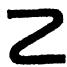
\includegraphics[keepaspectratio]{images/part003_0bad14cb.jpg}}

It follows from Proposition 2 that the lower envelope of a finite number of lower semi-continuous functions is again lower semi-continuous; but this is not in general true for the lower envelope of an infinite family of lower semi-continuous functions. For example, if r is any rational number, let \(f_{r}\) denote the function which is equal to 0 at r and equal to 1 for all real numbers \(x \neq r\) ; the lower envelope of the \(f_{r}\) is the function g which is equal to 0 for every rational number and 1 for every irrational number (``Dirichlet's function''), and this function is not lower semi-continuous at irrational points.

COROLLARY. The upper envelope of a family of continuous real-valued functions on a space X is lower semi-continuous on X.

In Chapter IX, § 1, no. 6, Proposition 5, we shall show that the converse of this proposition is true if X is uniformizable (and only in this case): every lower semi-continuous function on a uniformizable space is the upper envelope of a family of continuous functions.

PROPOSITION 3. A real-valued function \(f\) , defined on a topological space \(\mathbf{X}\) , is lower semi-continuous at a point \(a \in \mathbf{X}\) if and only if \(\liminf_{x \to a} f(x) = f(a)\) {[}or, equivalently, if and only if \(\liminf_{x \to a} f(x) \geqslant f(a)\) {]}.

The condition is necessary. For, given any \(h < f(a)\) , there is a neighbourhood \(V\) of \(a\) such that \(h < f(x)\) for all \(x \in V\) ; therefore

\[
h \leqslant \inf _ {x \in \mathbf {V}} f (x) \leqslant \liminf _ {x \rightarrow a} f (x)
\]

(§ 5, no. 6, formulae (12)), and so \(f(a) \leqslant \liminf_{x \to a} f(x)\) . The condition is sufficient; for if it is satisfied, then for each \(h < f(a)\) there is a neighbourhood \(V\) of \(a\) such that \(h \leqslant \inf_{x \in V} f(x)\) , and therefore \(f\) is lower semicontinuous at \(a\) .

PROPOSITION 4. Let \(f\) be any real-valued function defined on a dense subset \(A\) of a topological space \(X\) . If, for each \(x \in X\) , we put \(g(x) = \liminf_{y \to x, y \in A} f(y)\) , then \(g\) is lower semi-continuous on \(X\) .

For, given any \(h < g(x)\) , there is an open neighbourhood \(\mathbf{V}\) of \(x\) such that, for all \(z \in \mathbf{V} \cap \mathbf{A}\) , we have \(h < f(z)\) ; now \(\mathbf{V}\) is a neighbourhood of each of its points \(y\) ; thus we have \(\liminf_{z \to y, z \in \mathbf{A}} f(z) = g(y) \geqslant h\) for all \(y \in \mathbf{V}\) , and the result follows.

The function g is called the lower semi-continuous regularization of f.~We define the upper semi-continuous regularization of f similarly.

We may also define \(g\) as the greatest of the lower semi-continuous functions \(\varphi\) on \(\mathbf{X}\) which are such that \(\varphi(x) \leqslant f(x)\) for all \(x \in \mathbf{A}\) . If \(f\) is lower semi-continuous on \(\mathbf{A}\) , then \(g\) is an extension of \(f\) to \(\mathbf{X}\) , by Proposition 3.

\section{INFINITE SUMS AND PRODUCTS OF REAL NUMBERS}

Since every point of \(\mathbf{R}\) has a countable fundamental system of neighbourhoods (§ 1, no. 4, Corollary to Proposition 3), it follows that a family \((x_{t})\) of finite real numbers is summable in \(\mathbf{R}\) only if the set of indices \(t\) such that \(x_{t} \neq 0\) is countable (Chapter III, § 5, no. 2, Corollary to Proposition 1). The study of summable families in \(\mathbf{R}\) thus reduces essentially to the study of summable sequences. However, we shall later have to consider uncountable families \((x_{t})\) of finite real numbers, whose terms are functions of a parameter \(t\) ; it can happen that this family is summable for all t, but that the (countable) set of indices \(\iota\) such that \(x_{t} \neq 0\) depends on t. For this reason we shall not impose any hypothesis on the power of the index set in what follows.

\subsection{FAMILIES OF POSITIVE FINITE NUMBERS SUMMABLE IN R}

THEOREM 1. A family \((x_{t})\) of finite real numbers \(\geqslant 0\) is summable in \(\mathbf{R}\) if and only if the set of partial finite sums of the family is bounded above in \(\mathbf{R}\) . If so, the least upper bound of this set is the sum of the family \((x_{t})\) .

For each finite subset H of the index set I, let \(s_{H} = \sum_{i \in H} x_{i}\) ; since the \(x_{i}\) are \(\geqslant 0\) , the relation \(H \subset H'\) implies \(s_{H} \leqslant s_{H'}\) . In other words, the mapping \(H \to s_{H}\) is an increasing function on the directed set \(\mathfrak{F}(I)\) of finite subsets of I; therefore (§ 5, no. 2, Corollary to Theorem 2) it has a finite limit if and only if it is bounded above.

Remark. Let \((\mathrm{H}_{\lambda})\) be a family of finite subsets of I such that, for each finite subset H of I, there is an index \(\lambda\) such that \(H \subset H_{\lambda}\) ; then \((x_{t})\) is summable if and only if the family of the \(s_{H_{1}}\) is bounded above in R. In particular, let \((x_{n})\) be a sequence of finite real numbers \(\geqslant 0\) , and for each integer n let \(s_{n} = \sum_{p=0}^{n} x_{p}\) ; then the sequence \((x_{n})\) is summable in R if and only if, for one sequence of strictly increasing integers \((n_{k})\) , the partial sequence \((s_{n_{k}})\) is bounded above in R.

Examples. 1) For each number \(q\) such that \(0 \leqslant q < 1\) , the sequence \((q^n)\) ('geometric progression of ratio \(q''\) ) is summable in \(\mathbf{R}\) , since \(s_n = \frac{1 - q^{n+1}}{1 - q} \leqslant \frac{1}{1 - q}\) ; the sum of this sequence is \(\lim_{n \to \infty} s_n = \frac{1}{1 - q}\) .

\begin{enumerate}
\def\labelenumi{\arabic{enumi})}
\setcounter{enumi}{1}
\tightlist
\item
  Let \(a\) and \(b\) be two numbers such that \(0 \leqslant a < 1\) and \(0 \leqslant b < 1\) ; then the family \((a^{m}b^{n})_{(m,n) \in \mathbb{N} \times \mathbb{N}}\) is summable in \(\mathbb{R}\) . For each finite subset of \(\mathbf{N} \times \mathbf{N}\) is contained in a subset of the form \([0, p] \times [0, p]\) , and we have
\end{enumerate}

\[
\sum_ {m = 0} ^ {p} \sum_ {n = 0} ^ {p} a ^ {m} b ^ {n} = \left(\sum_ {m = 0} ^ {p} a ^ {m}\right) \left(\sum_ {n = 0} ^ {p} b ^ {n}\right) = \frac {1 - a ^ {p + 1}}{1 - a}. \frac {1 - b ^ {p + 1}}{1 - b} \leqslant \frac {1}{(1 - a) (1 - b)}.
\]

\begin{enumerate}
\def\labelenumi{\arabic{enumi})}
\setcounter{enumi}{2}
\tightlist
\item
  For each integer \(p > 1\) , the sequence \((n^{-p})\) ( \(n > 0\) ) is summable, since
\end{enumerate}

\[
s _ {2 ^ {n + 1}} - s _ {2 ^ {n}} = \sum_ {k = 1} ^ {2 ^ {n}} (2 ^ {n} + k) ^ {- p} <   2 ^ {n}. (2 ^ {n}) ^ {- p}
\]

and therefore, adding these inequalities together,

\[
s _ {2 ^ {n}} <   \frac {1}{1 - 2 ^ {1 - p}}.
\]

\begin{enumerate}
\def\labelenumi{\arabic{enumi})}
\setcounter{enumi}{3}
\tightlist
\item
The sequence \((1 / n)\) \((n > 0)\) is not summable in \(\mathbf{R}\) , since
\end{enumerate}

\[
s _ {2 ^ {n + 1}} - s _ {2 ^ {n}} = \sum_ {k = 1} ^ {2 ^ {n}} \frac {1}{2 ^ {n} + k} > \frac {2 ^ {n}}{2 ^ {n + 1}} = \frac {1}{2}
\]

and therefore, adding these inequalities together,

\[
s _ {2 ^ {n}} > n / 2
\]

so that the criterion of Theorem 1 is not satisfied.

\begin{enumerate}
\def\labelenumi{\arabic{enumi})}
\setcounter{enumi}{4}
\tightlist
\item
  Let \((\mathbf{I}_n)\) be a sequence of mutually disjoint non-empty open intervals, all contained in an interval of finite length \(l\) . The sum of the lengths of a finite number of intervals of this family is \(\leqslant l\) (§ 1, no. 5) and therefore the family of lengths of the \(\mathbf{I}_n\) is summable in \(\mathbf{R}\) , and its sum is \(\leqslant l\) .
\end{enumerate}

THEOREM 2 (Principle of comparison). Let \((x_{\iota})_{\iota\in I}\) and \((y_{\iota})_{\iota\in I}\) be two families of finite real numbers \(\geqslant 0\) , such that \(x_{\iota}\leqslant y_{\iota}\) for all \(\iota\) . If \((y_{\iota})\) is summable in \(\mathbb{R}\) then so is \((x_{\iota})\) , and we have \(\sum_{\iota}x_{\iota}\leqslant\sum_{\iota}y_{\iota}\) ; if in addition there is an index \(\chi\) such that \(x_{\chi}<y_{\chi}\) , then \(\sum_{\iota}x_{\iota}<\sum_{\iota}y_{\iota}\) .

The hypothesis implies that,

\[
\sum_ {\iota \in \mathbf {H}} x _ {\iota} \leqslant \sum_ {\iota \in \mathbf {H}} y _ {\iota},
\]

for every finite subset H of I and the first part of the theorem follows from this; the inequality relating the sums follows from the principle of extension of inequalities (§ 5, no. 2, Theorem 1). If \(x_{\chi} < y_{\chi}\) , then

\[
\sum_ {\iota} x _ {\iota} = x _ {\chi} + \sum_ {\iota \neq \chi} x _ {\iota} <   y _ {\chi} + \sum_ {i \neq x} y _ {\iota} = \sum_ {\iota} y _ {\iota}.
\]

This theorem provides the most commonly used criterion for deciding whether or not a sequence \((x_{n})\) of real numbers \(\geqslant0\) is summable in R: we try to compare the given sequence with a simpler sequence \((y_{n})\) of which we already know whether it is summable or not. If there exists a finite number a \textgreater{} 0 such that \(x_{n} \leqslant ay_{n}\) for all n from a certain point onwards, and if \((y_{n})\) is summable, then \((x_{n})\) is summable; if on the other hand there is a finite number b \textgreater{} 0 such that \(x_{n} \geqslant by_{n}\) for all n from a certain point onwards, and if \((y_{n})\) is not summable in R, then \((x_{n})\) is not summable in R. We shall see in a later volume how such comparison sequences may be obtained in the cases which arise most frequently.

Examples. 1) Let \(a\) be a finite real number \(>0\) , and consider the sequence \(\left(\frac{a^n}{n!}\right)\) ; let \(n_0\) be the smallest integer such that \(a < n_0\) . Then

for each \(n \geqslant n_0\) we have

\[
\frac {a ^ {n}}{n !} \leqslant \frac {a ^ {n _ {0}}}{n _ {0} !} \cdot \left(\frac {a}{n _ {0}}\right) ^ {n - n _ {0}};
\]

since \(q = \frac{a}{n_0} < 1\) , the sequence \((q^{n - n_0})\) is summable, and therefore so is the sequence \(\left(\frac{a^n}{n!}\right)\) .

\begin{enumerate}
\def\labelenumi{\arabic{enumi})}
\setcounter{enumi}{1}
\tightlist
\item
  Let \((a_{n})\) be a summable sequence of positive numbers. Since
\end{enumerate}

\[
\lim _ {n \rightarrow \infty} a _ {n} = 0,
\]

there exists an integer \(n_0\) such that \(a_n \leqslant 1\) whenever \(n \geqslant n_0\) . Consequently, for each \(n \geqslant n_0\) we have \(a_n^2 \leqslant a_n\) , and therefore the sequence \((a_n^2)\) is summable in \(\mathbb{R}\) . So is the sequence \((a_n^p)\) for each integer \(p > 1\) .

\begin{enumerate}
\def\labelenumi{\arabic{enumi})}
\setcounter{enumi}{2}
\tightlist
\item
  Let \(a\) and \(b\) be two numbers \(< 1\) ; then
\end{enumerate}

\[
\frac {1}{a ^ {m} + b ^ {n}} \leqslant \frac {1}{2 (\sqrt {a}) ^ {m} (\sqrt {b}) ^ {n}}
\]

and hence the family \(\left(\frac{1}{a^m + b^n}\right)\) is summable in \(\mathbf{R}\) .

COROLLARY. Let \((x_{i})_{i\in I}\) be a summable family of finite numbers \(\geqslant 0\) in R. If H is any subset of I, we have

\[
\sum_ {i \in \mathbf {H}} x _ {i} \leqslant \sum_ {i \in \mathbf {I}} x _ {i},
\]

and equality holds only if \(x_{i} = 0\) for all \(i \in \mathbb{C}\mathbb{H}\) .

\subsection{FAMILIES OF FINITE NUMBERS OF ARBITRARY SIGN SUMMABLE IN R}

THEOREM 3. Let \((x_{t})_{t\in I}\) be a family of finite real numbers; then the following statements are equivalent:

\begin{enumerate}
\def\labelenumi{\alph{enumi})}
\item
  The family \((x_{i})\) is summable in \(\mathbf{R}\) .
\item
  The family \((|x_{i}|)\) is summable in \(\mathbf{R}\) .
\item
  The set of finite partial sums of the family \((x_{t})\) is bounded in R.
\end{enumerate}

Let \(I_1\) be the set of all \(i \in I\) such that \(x_i \geq 0\) , and \(I_2\) the set of all \(i \in I\) such that \(x_i < 0\) . The family \((x_i)_{i \in I}\) {[}resp. \((|x_i|)_{i \in I}\) {]} is summable if and only if each of the families \((x_i)_{i \in I_1}\) and \((x_i)_{i \in I_2}\) {[}resp. \((|x_i|)_{i \in I_3}\) and \((|x_i|)_{i \in I_4}\) {]} is summable (Chapter III, § 5, no. 3, Propositions 2 and 3). Now it comes to the same thing to say that \((x_i)_{i \in I_1}\) is summable, or that \((|x_i|)_{i \in I_2}\) is summable, or that the set of finite partial sums of the family \((x_{i})_{i\in I_1}\) is bounded (no. 1, Theorem 1); and the same is true with \(I_1\) replaced by \(I_2\) . The theorem follows immediately.

Theorem 3 shows that the summability in R of a family of finite real numbers depends only on the summability of the family of their absolute values.

We recall (Chapter III, § 5, no. 5, Proposition 6) that if \((x_{t})\) and \((y_{t})\) are two summable families of finite real numbers, then the family \((x_{t} + y_{t})\) is summable and \(\sum_{i}(x_{t} + y_{t}) = \sum_{i}x_{t} + \sum_{i}y_{t}\) . Moreover, if \((x_{t})\) is a summable family of finite real numbers and \(a\) is any finite real number, then the family \((ax_{t})\) is summable in \(\mathbf{R}\) , and we have \(\sum_{i}ax_{t} = a\) . \(\sum_{i}x_{t}\) .

\subsection{PRODUCT OF TWO INFINITE SUMS}

PROPOSITION 1. If the families \((x_{\lambda})_{\lambda \in L}\) and \((y_{\mu})_{\mu \in M}\) of finite real numbers are summable in \(\mathbf{R}\) , then so is the family \((x_{\lambda}y_{\mu})_{(\lambda ,\mu)\in L\times M}\) and we have

\[
\sum_ {(\lambda , \mu) \in \mathbf {L} \times \mathbf {M}} x _ {\lambda} y _ {\mu} = (\sum_ {\lambda \in \mathbf {L}} x _ {\lambda}) (\sum_ {\mu \in \mathbf {M}} y _ {\mu}).\tag{1}
\]

Every finite subset of \(\mathbf{L} \times \mathbf{M}\) is contained in a finite subset of the form \(\mathbf{H} \times \mathbf{K}\) , where \(\mathbf{H}\) is a finite subset of \(\mathbf{L}\) and \(\mathbf{K}\) is a finite subset of \(\mathbf{M}\) . By hypothesis, there exists a number \(a > 0\) such that \(\sum_{\lambda \in \mathbf{H}} |x_{\lambda}| \leqslant a\) and \(\sum_{\mu \in \mathbf{K}} |y_{\mu}| \leqslant a\) for all finite subsets \(\mathbf{H}\) and \(\mathbf{K}\) of \(\mathbf{L}\) and \(\mathbf{M}\) respectively; therefore

\[
\sum_ {(\lambda , \mu) \in \mathbf {H} \times \mathbf {K}} | x _ {\lambda} y _ {\mu} | = (\sum_ {\lambda \in \mathbf {H}} | x _ {\lambda} |) (\sum_ {\mu \in \mathbf {K}} | y _ {\mu} |) \leqslant a ^ {2},
\]

and this shows that the family \((x_{\lambda}y_{\mu})\) is summable in \(\mathbf{R}\) , by Theorems 1 and 3. By associativity we can write {[}Chapter III, § 5, no. 3, formula (2){]}

\[
\sum_ {(\lambda , \mu) \in \mathbf {L} \times \mathbf {M}} x _ {\lambda} y _ {\mu} = \sum_ {\lambda \in \mathbf {L}} (\sum_ {\mu \in \mathbf {M}} x _ {\lambda} y _ {\mu}) = \sum_ {\lambda \in \mathbf {L}} x _ {\lambda} (\sum_ {\mu \in \mathbf {M}} y _ {\mu}) = (\sum_ {\lambda \in \mathbf {L}} x _ {\lambda}) (\sum_ {\mu \in \mathbf {M}} y _ {\mu});
\]

hence the result.

\subsection{FAMILIES MULTIPLIABLE IN R*}

In the multiplicative group \(\mathbb{R}^*\) of finite non-zero real numbers, a family \((x_{t})_{i\in I}\) can be multipliable only if \(\lim x_{t} = 1\) with respect to the filter of complements of finite subsets of I (Chapter III, § 5, no. 2, Proposition 1). In particular there can be only a finite number of indices \(i\) such that \(x_{t} < 0\) . We may therefore limit ourselves to considering only families \(x_{t}\) all of whose terms are strictly positive; it is then convenient to put \(x_{i} = i + u_{i}\) , where the \(u_{i}\) are subject to the inequalities \(-i < u_{i} < +\infty\) for all \(i\) . Since each point of \(\mathbf{R}^*\) has a countable fundamental system of neighbourhoods, the set of indices \(i\) such that \(u_{i} \neq 0\) is countable, if the family \((i + u_{i})\) is multipliable in \(\mathbf{R}^*\) .

THEOREM 4. The family \((1 + u_{t})\) is multipliable in \(\mathbb{R}^*\) if and only if the family \((u_{t})\) is summable in \(\mathbb{R}\) .

Lemma. (i) If \((a_{i})_{1\leqslant i\leqslant p}\) is a finite sequence of numbers \(>0\) , then

\[
\prod_ {i = 1} ^ {p} \left(1 + a _ {i}\right) \geqslant 1 + \sum_ {i = 1} ^ {p} a _ {i}.\tag{2}
\]

\begin{enumerate}
\def\labelenumi{(\roman{enumi})}
\setcounter{enumi}{1}
\tightlist
\item
  If also \(a_i < 1\) for each \(i\) , then
\end{enumerate}

\[
\prod_ {i = 1} ^ {p} \left(\mathrm{I} - a _ {i}\right) \geqslant \mathrm{I} - \sum_ {i = 1} ^ {p} a _ {i}.\tag{3}
\]

These inequalities are clear if \(p = 1\) , and are proved by induction on \(p\) . If

\[
\prod_ {i = 1} ^ {p - 1} \left(\mathrm{I} + a _ {i}\right) \geqslant \mathrm{I} + \sum_ {i = 1} ^ {p - 1} a _ {i},
\]

we have

\[
\prod_ {i = 1} ^ {p} \left(\mathrm{I} + a _ {i}\right) \geqslant \left(\mathrm{I} + a _ {p}\right) \left(\mathrm{I} + \sum_ {i = 1} ^ {p - 1} a _ {i}\right) = \mathrm{I} + \sum_ {i = 1} ^ {p} a _ {i} + a _ {p}. \sum_ {i = 1} ^ {p - 1} a _ {i} \geqslant \mathrm{I} + \sum_ {i = 1} ^ {p} a _ {i}.
\]

Again, if

\[
\prod_ {i = 1} ^ {p - 1} \left(\mathrm{I} - a _ {i}\right) \geqslant \mathrm{I} - \sum_ {i = 1} ^ {p - 1} a _ {i},
\]

we have

\[
\prod_ {i = 1} ^ {p} \left(\mathrm{I} - a _ {i}\right) \geqslant \left(\mathrm{I} - a _ {p}\right) \left(\mathrm{I} - \sum_ {i = 1} ^ {p - 1} a _ {i}\right) = \mathrm{I} - \sum_ {i = 1} ^ {p} a _ {i} + a _ {p}. \sum_ {i = 1} ^ {p - 1} a _ {i} \geqslant \mathrm{I} - \sum_ {i = 1} ^ {p} a _ {i}.
\]

Having proved the lemma, we note that if the family \((\mathbf{I} + u_{t})\) is multipliable then so are the families \((\mathbf{I} + u_{t}^{+})\) and \((\mathbf{I} - u_{t}^{-})\) , since \(\mathbf{R}^*\) is a complete group (Chapter III, § 5, no. 3, Proposition 2); and conversely, if the families \((\mathbf{I} + u_{t}^{+})\) and \((\mathbf{I} - u_{t}^{-})\) are multipliable, then so is \((\mathbf{I} + u_{t})\) (Chapter III, § 5, no. 3, Proposition 3). We need therefore consider only the cases in which all the \(u_{t}\) are \(\geqslant 0\) and in which they are all \(\leqslant 0\) .

Suppose first that \(u_{t} \geqslant 0\) for all \(t\) . If the family \((1 + u_{t})\) is multipliable, then for each \(\varepsilon > 0\) there is a finite subset \(J\) of the index set in \(I\) such that, for each finite subset \(H\) of \(I\) disjoint from \(J\) , we have \(\mathbf{I} \leqslant \prod_{i \in \mathbf{H}} (\mathbf{I} + u_i) \leqslant \mathbf{I} + \varepsilon\) ; by (2) it follows that \(\sum_{i \in \mathbf{H}} u_i \leqslant \varepsilon\) , which shows that \((u_i)\) is summable in \(\mathbf{R}\) by virtue of Cauchy's criterion (Chapter III, § 5, no. 2, Theorem I).

Conversely, suppose that \((u_{t})\) is summable in \(\mathbf{R}\) . For each \(\varepsilon\) such that \(0 < \varepsilon < 1\) , there is a finite subset \(J\) of \(I\) such that, for each finite subset \(H\) of \(I\) disjoint from \(J\) , we have \(0 \leqslant \sum_{t \in H} u_{t} \leqslant \varepsilon\) . By (3), we have therefore \(\prod_{t \in H} (I - u_{t}) \geqslant I - \varepsilon\) ; but since \(I + u \leqslant \frac{I}{I - u}\) for every number \(u\) such that \(0 \leqslant u < 1\) , it follows that

\[
\mathrm{I} \leqslant \prod_ {i \in \mathrm{H}} (\mathrm{I} + u _ {i}) \leqslant \frac {\mathrm{I}}{\mathrm{I} - \varepsilon},
\]

and this shows that \((\mathbf{I} + u_{t})\) is multipliable (Cauchy's criterion).

The proof is similar when all the \(u_{i}\) are \(\leqslant 0\) . To show that \((u_{i})\) is summable if \((1 + u_{i})\) is multipliable, use formula (2) and the inequality \(1 - u \leqslant \frac{1}{1 + u}\) ( \(0 \leqslant u < 1\) ); to show that \((1 + u_{i})\) is multipliable if \((u_{i})\) is summable, use formula (3).

In Chapter V (§ 4), the topological study of the group \(\mathbf{R}^*\) will enable us to give another criterion for multipliability of a family in \(\mathbf{R}^*\) with the help of the logarithmic function; in a later volume we shall establish the equivalence of this criterion with the one above, using the differential properties of the logarithm.

\subsection{\texorpdfstring{SUMMABLE FAMILIES AND MULTIPLIABLE FAMILIES IN \(\overline{\mathbf{R}}\)}{SUMMABLE FAMILIES AND MULTIPLIABLE FAMILIES IN \textbackslash overline\{\textbackslash mathbf\{R\}\}}}

On the interval \([0, +\infty]\) of \(\overline{\mathbf{R}}\) , addition is an associative and commutative law of composition (§ 4, no. 3); hence the notion of a summable family of numbers in this interval is defined (Chapter III, § 5, no. 1, Remark 3).

PROPOSITION 2. Every family \((x_{\mathfrak{t}})\) of real numbers \(\geqslant 0\) is summable in \(\overline{\mathbf{R}}\) . For the mapping \(\mathbf{H} \to s_{\mathbf{H}}\) of the directed set \(\mathfrak{F}(\mathbf{I})\) into \(\overline{\mathbf{R}}\) is increasing; hence (§ 5, no. 2, Theorem 2) has a limit.

The same reasoning shows that every family of real numbers \(\leqslant 0\) is summable in \(\overline{\mathbf{R}}\) .

Similarly, multiplication is an associative and commutative law of composition on each of the intervals \([0, 1]\) and \([1, +\infty]\) of \(\overline{R}\) , and therefore the notion of a multipliable family is defined on each of these intervals.

PROPOSITION 3. Every family \((1 + u_{t})\) {[}resp. \((1 - u_{t})]\) of numbers \(\geqslant 1\) (resp. \(\geqslant 0\) and \(\leqslant 1\) ) is multipliable in \(\overline{\mathbf{R}}\) .

Same proof as for Proposition 2.

COROLLARY. The product \(\prod_{i} (1 + u_i) [\text{resp. } \prod_{i} (1 - u_i))\) of numbers \(\geqslant 1\) (resp. \(>0\) and \(\leqslant 1\) ) is equal to \(+\infty\) (resp. 0) if and only if \(\sum_{i} u_i = +\infty\) . For if \(\sum_{i} u_i\) is finite then \(\prod_{i} (1 + u_i)\) and \(\prod_{i} (1 - u_i)\) are in \(\mathbf{R}^*\) , and conversely (no. 4, Theorem 4).

Remark. The theorem of associativity (Chapter III, § 5, no. 3, Theorem 2) remains valid when G is replaced by \(\overline{\mathbf{R}}\) and the \(x_{i}\) are assumed to be \(\geqslant 0\) . This is clear if \(\sum_{i \in I} x_{i}\) is finite. Suppose, on the contrary, that \(\sum_{i \in I} x_{i} = +\infty\) . Then for each finite \(a > 0\) there is a finite subset H of I such that \(\sum_{i \in H} x_{i} \geqslant a\) . Let K be a finite subset of L such that \(H \subset \bigcup_{\lambda \in K} I_{\lambda}\) ; then since \(s_{\lambda} \geqslant \sum_{i \in I_{\lambda} \cap H} x_{i}\) for all \(\lambda \in K\) , we have

\[
\sum_ {\lambda \in \mathbf {K}} s _ {\lambda} \geqslant \sum_ {i \in \mathbf {H}} x _ {i} \geqslant a,
\]

which shows that \(\sum_{\lambda \in L} s_{\lambda} = +\infty\) . We leave to the reader the task of formulating the analogous proposition for multipliable families of numbers in \([0, 1]\) or in \([1, +\infty]\) .

\subsection{INFINITE SERIES AND INFINITE PRODUCTS OF REAL NUMBERS}

A series of finite real numbers is simply said to be convergent if it is convergent in R.

DEFINITION 1. A series of finite real numbers is said to be absolutely convergent if the series of absolute values of its terms is convergent.

PROPOSITION 4. A series of finite real numbers is commutatively convergent if and only if it is absolutely convergent.

This follows from Chapter III, § 5, no. 7, Proposition 9 and from Theorem 3 of no. 2.

In other words, if \((u_{n})\) is a sequence of finite real numbers, it comes to the same thing to say that the series whose general term is \(u_{n}\) is commutatively convergent, or that it is absolutely convergent, or that the sequence \((u_{n})\)

is summable in \(\mathbf{R}\) . All the properties of summable families proved in Chapter III, § 5 therefore apply to absolutely convergent series. In particular, if the series whose general term is \(u_{n}\) is absolutely convergent, then the sum \(\sum_{n\in\mathbf{H}} u_{n}\) exists for all subsets \(\mathbf{H}\) of \(\mathbf{N}\) ; and, if \((\mathbf{H}_{p})\) is a partition of \(\mathbf{N}\) , we have

\[
\sum_ {n = 0} ^ {\infty} u _ {n} = \sum_ {p} \left(\sum_ {n \in \mathrm{H} _ {p}} u _ {n}\right)
\]

(associativity of absolutely convergent series).

As we have already remarked in Chapter III, § 5, a series of real numbers can be convergent without being commutatively convergent, that is, without being absolutely convergent.

Example. Alternating series. A series defined by a sequence \((u_n)\) of finite real numbers is called alternating if \(u_n = (-1)^n v_n\) , where \(v_n \geqslant 0\) for all \(n\) . Let us show that a sufficient condition for the convergence of such a series is that the sequence \((v_n)\) decreases and has \(0\) as its limit. For if \(s_n\) denotes

\[
\sum_ {p = 0} ^ {n} u _ {p},
\]

the hypothesis that \((v_{n})\) is decreasing implies that

\[
s _ {2 n + 1} \leqslant s _ {2 n + 3} \leqslant s _ {2 n + 2} \leqslant s _ {2 n}
\]

for all \(n \geqslant 0\) . The sequence \((s_{2n})\) {[}resp. \((s_{2n+1})\) {]} is decreasing and bounded below (resp. increasing and bounded above) and therefore has a finite limit a (resp. b), and \(b \leqslant a\) ; since

\[
a - b = \lim _ {n \rightarrow \infty} (s _ {2 n} - s _ {2 n + 1}) = \lim _ {n \rightarrow \infty} v _ {2 n + 1} = 0,
\]

the assertion is proved.

If we take for example \(v_{n}=1/n\) , the conditions above are satisfied, and therefore the series whose general term is \((-1)^{n}/n\) (the ``alternating harmonic series'') is convergent. We have seen in no. 1 that the series whose general term is 1/n (the ``harmonic series'') is not convergent, and thus the alternating harmonic series is not absolutely convergent.

We recall (Chapter III, § 5, no. 6, Proposition 7) that, if \((u_n)\) and \((v_n)\) are two convergent series of finite real numbers, then the series \((u_n + v_n)\) is convergent, and

\[
\sum_ {n = 0} ^ {\infty} \left(u _ {n} + v _ {n}\right) = \sum_ {n = 0} ^ {\infty} u _ {n} + \sum_ {n = 0} ^ {\infty} v _ {n};
\]

also, if the series \((u_{n})\) is convergent then the series \((au_{n})\) is convergent for all finite real numbers \(a\) , and \(\sum_{n=0}^{\infty} au_{n} = a\) . \(\sum_{n=0}^{\infty} u_{n}\) .

Finally, if the series \((u_n)\) and \((v_n)\) are convergent, and if \(u_n \leqslant v_n\) for all \(n\) , we have \(\sum_{n=0}^{\infty} u_n \leqslant \sum_{n=0}^{\infty} v_n\) by the principle of extension of inequalities (§ 5, no. 2, Theorem 1).

It should be noted that, if we suppose the series \((v_{n})\) to be convergent but not absolutely convergent, and if \(|u_{n}| \leqslant |v_{n}|\) for each n, we can by no means infer that the series \((u_{n})\) is convergent, as is seen by taking \(u_{n} = |v_{n}|\) .

An infinite product of finite non-zero real numbers is said simply to be convergent if it is convergent in \(\mathbf{R}^*\) ; its value is then a finite non-zero real number.

DEFINITION 2. An infinite product whose general factor is \(1 + u_{n}\) is said to be absolutely convergent if the product whose general factor is \(1 + |u_{n}|\) is convergent.

PROPOSITION 5. An infinite product of finite real numbers is commutatively convergent if and only if it is absolutely convergent.

This follows from Chapter III, § 5, no. 7, Proposition 9, and from Theorem 4 above.

Moreover, the product whose general factor is \(1 + u_{n}\) is absolutely convergent if and only if the series whose general term is \(u_{n}\) is absolutely convergent.

A product of non-zero real numbers can be convergent without being commutatively convergent, i.e.~without being absolutely convergent.

Example. If we take \(u_{2n-1} = -\frac{1}{n}\) and \(u_{2n} = \frac{1}{n}\) for \(n \geqslant 2\) , the product \((1 + u_n)\) is not absolutely convergent, since the series \((u_n)\) is not absolutely convergent; but since

\[
\begin{array}{l} \prod_ {p = 3} ^ {n} (1 + u _ {p}) = \prod_ {p = 2} ^ {n} \left(1 - \frac {1}{p ^ {2}}\right), \\ \text { and } \quad \prod_ {p = 3} ^ {2 n + 1} (1 + u _ {p}) = \left(1 - \frac {1}{n + 1}\right) \prod_ {p = 2} ^ {n} \left(1 - \frac {1}{p ^ {2}}\right), \end{array}
\]

it follows from Theorem 4 that the product is convergent and that its value is

\[
\prod_ {n = 2} ^ {\infty} \left(1 - \frac {1}{n ^ {2}}\right).
\]

\pandocbounded{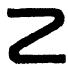
\includegraphics[keepaspectratio]{images/part003_4cdcc444.jpg}}

Moreover, it should be observed that the convergence of the series whose general term is \(u_{n}\) is neither necessary nor sufficient for the convergence of the product whose general factor is \(1 + u_{n}\) (see Exercises 21 and 22).

\section{USUAL EXPANSIONS OF REAL NUMBERS; THE POWER OF R}

\subsection{APPROXIMATIONS TO A REAL NUMBER}

DEFINITION 1. Given a number \(\varepsilon > 0\) , a real number \(r\) is said to be an approximation to within \(\varepsilon\) to a real number \(x\) , if \(|x - r| \leqslant \varepsilon\) ; \(r\) is said to be an approximation by defect if \(r \leqslant x\) , by excess if \(r \geqslant x\) .

Let A be a dense subset of R. For each \(x \in R\) and each \(\varepsilon > 0\) there is an approximation by defect (resp. excess) to x to within \(\varepsilon\) belonging to A, since the interval \(]x - \varepsilon, x[\) (resp. \(]x, x + \varepsilon[\) ) contains at least one point of A. If we now consider a given strictly decreasing sequence ( \(\varepsilon_{n}\) ) of numbers \textgreater{} 0, tending to 0, and if \(r_{n}\) is an approximation to x to within \(\varepsilon_{n}\) , then the sequence ( \(r_{n}\) ) has x as limit as n tends to infinity.

In the case where A is a subgroup of the additive group R, and we restrict the \(\varepsilon_{n}\) to belong to A, we can define canonically for each \(x \in R\) a sequence \((r_{n})\) of approximations to x by defect, belonging to A.

For by Archimedes' axiom (§ 2, no. 1, Theorem 1), the set of integers \(p\) such that \(p\varepsilon_n \leqslant x\) has a greatest element \(p_n\) ; in other words, there is a unique integer \(p_n\) such that

\[
p _ {n} \varepsilon_ {n} \leqslant x <   (p _ {n} + 1) \varepsilon_ {n}.\tag{1}
\]

Since \(|x - p_n\varepsilon_n| \leqslant \varepsilon_n\) , it follows that \(p_n\varepsilon_n\) is an approximation to \(x\) to within \(\varepsilon_n\) by defect, and belongs to A by hypothesis; similarly \((p_n + 1)\varepsilon_n\) is an approximation to \(x\) to within \(\varepsilon_n\) by excess, belonging to A, and the two sequences \((p_n\varepsilon_n)\) and \(((p_n + 1)\varepsilon_n)\) have \(x\) as their limit.

\subsection{EXPANSIONS OF REAL NUMBERS RELATIVE TO A BASE SEQUENCE}

We shall limit ourselves to studying the case where \(\varepsilon_{n} = 1 / d_{n}\) , where \((d_n)\) is a strictly increasing sequence of integers such that \(d_0 = 1\) and \(d_n\) is a multiple of \(d_{n-1}\) for \(n \geqslant 1\) . Let \(a_n = d_n / d_{n-1}\) ( \(n \geqslant 1\) ): \(a_n\) is an integer \(>1\) . In this case, the sequence of approximations by defect \(r_n = p_n / d_n\) is increasing, for \(p_n\) is the largest integer such that \(p_n / d_n \leqslant x\) ;

but we have

\[
\frac {p _ {n - 1}}{d _ {n - 1}} = \frac {p _ {n - 1} a _ {n}}{d _ {n}} \leqslant x <   \frac {p _ {n - 1} + 1}{d _ {n - 1}} = \frac {p _ {n - 1} a _ {n} + a _ {n}}{d _ {n}}
\]

so that \(a_{n}p_{n - 1}\leqslant p_{n} <   a_{n}p_{n - 1} + a_{n},\) and therefore \(r_{n - 1}\leqslant r_n\leqslant x.\) Let

\[
p _ {n} = a _ {n} p _ {n - 1} + u _ {n};\tag{2}
\]

then \(0 \leqslant u_n < a_n\) , which is equivalent to \(0 \leqslant u_n \leqslant a_n - 1\) , since \(u_n\) is an integer. Hence

\[
r _ {n} = r _ {n - 1} + \frac {u _ {n}}{d _ {n}} = p _ {0} + \sum_ {k = 1} ^ {n} \frac {u _ {k}}{d _ {k}},\tag{3}
\]

and, since \(x = \lim_{n\to \infty}r_n,\)

\[
x = p _ {0} + \sum_ {n = 1} ^ {\infty} \frac {u _ {n}}{d _ {n}}.\tag{4}
\]

The series on the right-hand side of (4), whose sum is \(x\) , is called the expansion of \(x\) relative to the base sequence \((d_n)\) . All the coefficients \(u_n\) are \(\geqslant 0\) ; \(p_0\) is, by definition, the largest integer \(p\) such that \(p \leqslant x\) ; it is called the integral part of \(x\) , and is often denoted by {[}x{]}.

\subsection{DEFINITION OF A REAL NUMBER BY MEANS OF ITS EXPANSION}

Conversely, suppose we are given an integer \(q_0\) and a sequence \((v_n)\) ( \(n \geqslant 1\) ) of integers such that \(0 \leqslant v_n \leqslant a_n - 1\) ; we ask whether there is a number \(x\) whose expansion (4) is such that \(p_0 = q_0\) and \(u_n = v_n\) for all \(n\) . If such a number exists it is unique, because it is equal to \(q_0 + \sum_{n=1}^{\infty} \frac{v_n}{d_n}\) .

For each integer \(m > 0\) we have (by the principle of comparison)

\[
\sum_ {n = m + 1} ^ {\infty} \frac {v _ {n}}{d _ {n}} \leqslant \sum_ {n = m + 1} ^ {\infty} \frac {a _ {n} - 1}{d _ {n}} = \sum_ {n = m + 1} ^ {\infty} \left(\frac {1}{d _ {n - 1}} - \frac {1}{d _ {n}}\right) = \frac {1}{d _ {m}}
\]

and the extreme left-hand and right-hand terms are equal only if \(v_{n} = a_{n} - 1\) for each \(n > m\) (§ 7, no. 1, Theorem 2). Hence the series whose general term is \(\frac{v_n}{d_n}\) is convergent; moreover, if \(x = q_0 + \sum_{n=1}^{\infty} \frac{v_n}{d_n}\) , we have

\[
s _ {m} = q _ {0} + \sum_ {n = 1} ^ {m} \frac {v _ {n}}{d _ {n}} \leqslant x \leqslant s _ {m} + \frac {1}{d _ {m}}
\]

and \(x = s_m + \frac{1}{d_m}\) only if \(v_n = a_n - 1\) for each \(n > m\) . Since \(s_m\) is a fraction with denominator \(d_m\) , the approximation \(r_m\) to \(x\) to within \(1/d_m\) by defect is equal to \(s_m\) or \(s_m + \frac{1}{d_m}\) ; and the latter alternative can occur only if \(v_{n} = a_{n} - 1\) for all \(n > m\) . Thus:

\begin{enumerate}
\def\labelenumi{(\roman{enumi})}
\item
  There is an infinity of values of \(n\) such that \(v_{n} < a_{n} - 1\) : then the series \(q_{0} + \sum_{n=1}^{\infty} \frac{v_{n}}{d_{n}}\) is identical with the expansion of its sum \(x\) .
\item
  There is an integer \(m \geqslant 0\) such that \(v_{n} = a_{n} - 1\) whenever \(n > m\) , and \(v_{m} < a_{m} - 1\) (if \(m > 0\) ); then the sum \(x\) of the series \(q_{0} + \sum_{n=1}^{\infty} \frac{v_{n}}{d_{n}}\) is equal to the rational number
\end{enumerate}

\[
q _ {0} + \sum_ {n = 1} ^ {m} \frac {v _ {n}}{d _ {n}} + \frac {1}{d _ {m}}\tag{5}
\]

which is of the form \(k/d_{m}\) (k an integer); the expansion of x is identical with the series (5), in which all the terms with indices \textgreater{} m are zero; such an expansion is said to be terminating, or to terminate. The series

\[
q _ {0} + \sum_ {n = 1} ^ {\infty} \frac {v _ {n}}{d _ {n}} = q _ {0} + \sum_ {n = 1} ^ {m} \frac {v _ {n}}{d _ {n}} + \sum_ {n = m + 1} ^ {\infty} \frac {a _ {n} - 1}{d _ {n}}\tag{6}
\]

is called the improper expansion of the number x.

Conversely, let x be a rational number which can be written in the form of a fraction with denominator \(d_{n}\) for some value of n.~Let m be the smallest integer such that x is of the form \(k/d_{m}\) (k an integer); we have \(r_{n}<x\) for n\textless m, and \(r_{m}=x\) , and therefore the expansion of x is of the form (5), and x has an improper expansion given by (6); moreover this improper expansion is unique.

A rational number, written in its irreducible form \(p / q\) , is equal to a fraction with denominator \(d_n\) if and only if \(q\) divides \(d_n\) (the number \(m\) will therefore be the smallest integer \(n\) such that \(q\) divides \(d_n\) ). It can happen that every rational number has this property (for a suitably chosen \(n\) ): this will be the case if and only if every integer \(> 0\) divides some \(d_n\) , e.g., if \(d_n = n!\) . If the \(d_n\) have this property, then a number is rational if and only if its expansion, relative to the sequence \((d_n)\) , terminates.

To summarize: to every sequence \(s\) whose initial term \(q_{0}\) is an arbitrary integer, and whose term \(v_{n}(n \geqslant 1)\) is such that \(0 \leqslant v_{n} \leqslant a_{n} - 1\) , corresponds a real number equal to \(q_{0} + \sum_{n=1}^{\infty} \frac{v_{n}}{d_{n}}\) ; if \(I_{n}\) denotes the interval \([0, a_{n} - 1]\) of \(N\) , we thus define a mapping \(\varphi\) of \(X = Z \times \prod_{n=1}^{\infty} I_{n}\) onto the real line \(R\) ; moreover the equation \(\varphi(s) = x\) , where \(x \in R\) is given, has one solution if \(x\) is not a fraction with denominator \(d_{n}\) (for some \(n\) ), and two solutions otherwise.

\subsection{COMPARISON OF EXPANSIONS}

If we know the expansions of two distinct real numbers \(x\) and \(y\) , we can determine whether \(x < y\) or \(x > y\) .

Let \(x = p_0 + \sum_{n=1}^{\infty} u_n / d_n\) , \(y = q_0 + \sum_{n=1}^{\infty} v_n / d_n\) be the expansions of \(x\) and \(y\) . If \(p_0 < q_0\) then \(x < y\) , since

\[
p _ {0} \leqslant x <   p _ {0} + 1 \leqslant q _ {0} \leqslant y.
\]

More generally, suppose that \(p_0 = q_0\) and \(u_n = v_n\) for \(1 \leqslant n \leqslant m\) , but that \(u_m < v_m\) ; if

\[
r _ {n} = p _ {0} + \sum_ {k = 1} ^ {n} u _ {k} / d _ {k}, \quad s _ {n} = q _ {0} + \sum_ {k = 1} ^ {n} v _ {k} / d _ {k},
\]

then \(r_n = s_n\) for \(n < m\) , and since \(u_m + 1 \leqslant v_m\) , \(r_m + \frac{1}{d_m} \leqslant s_m\) ; but \(r_m \leqslant x < r_m + \frac{1}{d_m} \leqslant s_m \leqslant y\) , hence again we have \(x < y\) . In other words, the order of \(x\) and \(y\) is the same as the order of the first two distinct terms of their respective expansions.

It follows that, if \(p_{0}=q_{0}\) and \(u_{n}=v_{n}\) for n\textless m, then the first m terms of the expansion of every number z belonging to the closed interval with end-points x and y are the same as those of the expansions of x and y.

We remark also that, in this case, we have \(|y - x| \leqslant \frac{1}{d_{m-1}}\) . If we endow

Z and the intervals \(I_{n}\) with the discrete topology, it follows that the mapping \(\varphi\) defined above is continuous on the product space X.

\subsection{EXPANSIONS TO BASE A}

The most important base sequences are those for which \(d_{n}=a^{n}\) , where a is an integer \textgreater1; a is then said to be the base number (or simply the base) of the corresponding expansions. For numerical calculations, expansions to base 10, which are called decimal expansions, are used; also expansions to base 2 (dyadic expansions) and base 3 (triadic expansions) are often used.

To represent the approximations by defect \(r_n\) to a number \(x \geqslant 0\) , in its expansion to base \(a\) , the following symbolism is employed: each integer \(u\) such that \(0 \leqslant u \leqslant a - 1\) is denoted by a particular sign; if

\[
r _ {n} = p _ {0} + \sum_ {k = 1} ^ {n} \frac {u _ {k}}{d _ {k}},
\]

we first write down, with the aid of these signs, the representation to base \(a\) of the integer \(p_{0}=[x]\geqslant0\) (Set Theory, Chapter III, § 5, no. 7), then we put a point (``decimal point'') and we write

successively the signs representing the numbers \(u_1, u_2, \ldots, u_n\) . If \(S\) is the symbol thus obtained, it is customary to write \(x = S \ldots\) , by abuse of language. It should be understood once and for all that such a relation is only an abbreviated method of indicating that the right-hand side is the approximation to \(x\) to within \(1/a^n\) by defect.

For negative numbers the established usage is different: we write an approximation to \(x' = -x > 0\) in the symbolism described above, and precede it by the sign ``-''; it is thus an approximation to \(x\) to within \(1/a^n\) by excess that is so denoted.

This usage has its inconveniences for numerical calculations. In the notation for negative logarithms the same symbolism is adopted as for positive numbers, by putting a bar over the integral part, to indicate that it is equal to the negative of the number written.

\subsection{THE POWER OF R}

We have \(\mathbf{R} = \bigcup_{n\in \mathbf{Z}}[n,n + 1[,\) and all the intervals \([n,n + 1[\) are equipotent to \([0,1[\) . Since \([0,1[\) is an infinite set it follows that \(\mathbf{R}\) is equipotent to the interval \([0,1[\) . By considering the dyadic expansion of the numbers of the interval \([0,1[\) we shall show that this interval is equipotent to the set S of all sequences \((u_n)\) in which each term is equal to 0 or 1.

First, it is equipotent to the subset \(S'\) of \(S\) consisting of sequences \((u_n)\) such that \(u_n = 0\) for an infinity of values of \(n\) . On the other hand, the complement \(S''\) of \(S'\) in \(S\) is equipotent to the set of all improper expansions of rational numbers which are equal to a fraction with denominator \(2^n\) ; these numbers form a subset of \(Q\) , hence the set of them is countable and therefore so is \(S''\) . Since \(S'\) is infinite, it is equipotent to \(S\) , hence the result.

Now S is equipotent to \(\mathfrak{P}(\mathbf{N})\) ; for we can define a bijection of \(\mathfrak{P}(\mathbf{N})\) onto S by mapping each subset A of N to the sequence \((u_n)\) such that \(u_n = 0\) if \(n \in A\) and \(u_n = 1\) if \(n \in \mathbb{C}A\) . We have thus proved:

THEOREM 1 (Cantor). The set of real numbers is equipotent to the set of all subsets of a countably infinite set.

COROLLARY. The set of real numbers has a cardinal strictly greater than the cardinal of a countable set.

A set equipotent to R is said to have the power of the continuum. By Proposition 1 of § 4, no. 1, every interval which contains more than one point has the power of the continuum. Again, the complement of a countable subset of R has the power of the continuum in particular, the set of all irrational numbers has the power of the continuum.

\BourbakiExercises
\BourbakiExerciseGroup

\begin{enumerate}
\def\labelenumi{\arabic{enumi})}
\tightlist
\item
  A topology \(\mathfrak{G}\) on an ordered commutative group \(\mathbf{G}\) is said to be compatible with the ordered group structure of \(\mathbf{G}\) if it is compatible with the group structure of \(\mathbf{G}\) and if in addition the set \(\mathbf{G}_{+}\) of elements \(x \geqslant 0\) in \(\mathbf{G}\) is closed with respect to \(\mathfrak{G}\) .
\end{enumerate}

\begin{enumerate}
\def\labelenumi{\alph{enumi})}
\item
  Let \(\mathfrak{G}\) be a Hausdorff topology compatible with the ordered group structure of \(\mathbf{G}\) , and let \(\hat{\mathbf{G}}\) be the completion of \(\mathbf{G}\) (with respect to \(\mathfrak{G}\) ). In the group \(\hat{\mathbf{G}}\) , the closure \(\mathbf{P}\) of \(\mathbf{G}_{+}\) is such that \(y - x \in \mathbf{P}\) is a pre-ordering compatible with the group structure of \(\hat{\mathbf{G}}\) .
\item
  Let \(\theta\) be an irrational number, and consider the ordering on \(\mathbf{Q}^2\) for which the set of positive elements consists of (0, 0) and all pairs \((x, y)\) such that \(y - \theta x \geqslant 0\) . With respect to this ordering, \(\mathbf{Q}^2\) is a linearly ordered group, and the topology on \(\mathbf{Q}^2\) which is the product of the topology of the rational line by itself is compatible with this ordered group structure. But on \(\hat{\mathbf{G}} = \mathbb{R}^2\) , the relation \(y - x \in \mathbf{P} = \overline{\mathbf{G}}_+\) is not an ordering.
\item
  On a linearly ordered group G, the topology \(\mathfrak{C}_{0}(\mathbf{G})\) (Chapter I, § 2, Exercise 5) is the coarsest of all topologies compatible with the ordered group structure (distinguish two cases, according as the set of all \(x > 0\) has or has not a smallest element). Every topology on G which is compatible with the group structure of G and is finer than \(\mathfrak{C}_{0}(\mathbf{G})\) is compatible with the ordered group structure of G, and the mapping \(x \to x^{+}\) is continuous with respect to such a topology. This mapping is uniformly continuous with respect to \(\mathfrak{C}_{0}(\mathbf{G})\) , but not necessarily with respect to a group topology \(\mathfrak{C}\) strictly finer than \(\mathfrak{C}_{0}(\mathbf{G})\) {[}see b){]}.
\end{enumerate}

\begin{enumerate}
\def\labelenumi{\arabic{enumi})}
\setcounter{enumi}{1}
\tightlist
\item
  \begin{enumerate}
  \def\labelenumii{\alph{enumii})}
  \tightlist
  \item
    Let G be a lattice-ordered commutative group. For each \(x \geqslant 0\) in G, let \(\mathbf{I}(x)\) denote the interval \([-x, x]\) in G. A non-empty family \((c_{\alpha})\) of elements \(\geqslant 0\) in G is such that the intervals \(\mathbf{I}(c_{\alpha})\)
  \end{enumerate}
\end{enumerate}

form a fundamental system of neighbourhoods of 0 for a topology \(\mathfrak{G}\) on G compatible with the group structure of G if and only if the set of \(c_{\alpha}\) is directed (with respect to the relation \(\geqslant\) ) and for each \(\alpha\) there exists \(\beta\) such that \(2c_{\beta} \leqslant c_{\alpha}\) . If these conditions are satisfied, the mapping \(x \to x^{+}\) of G into G is uniformly continuous. \(\mathfrak{G}\) is Hausdorff if and only if \(\inf c_{\alpha} = 0\) ; and in this case \(\mathfrak{G}\) is compatible with the ordered group structure of G.

\begin{enumerate}
\def\labelenumi{\alph{enumi})}
\setcounter{enumi}{1}
\item
  On the group \(G = Z^{N}\) , the product of a countable infinity of linearly ordered groups Z, there is no non-discrete topology defined by the procedure of a), but the product of the discrete topologies on the factors Z is a topology on G, compatible with the ordered group structure of G, which is Hausdorff and not discrete.
\item
  On a linearly ordered group G the only Hausdorff topology defined by the procedure of a) is the topology \(\mathcal{G}_{0}(G)\) (Chapter I, § 2, Exercise 5).
\end{enumerate}

\begin{enumerate}
\def\labelenumi{\arabic{enumi})}
\setcounter{enumi}{2}
\tightlist
\item
  Let G be a lattice-ordered commutative group, and let M be the semigroup of major subsets of G. Every subset of M which is bounded above (resp. below) has a least upper bound (resp. greatest lower bound), and G can be canonically identified with a subset of M. Let G' denote the largest subgroup of M (the set of all symmetrizable elements of M).
\end{enumerate}

\begin{enumerate}
\def\labelenumi{\alph{enumi})}
\tightlist
\item
  Consider a topology \(\mathcal{G}\) on \(\mathbf{G}\) defined by the process of Exercise 2 \(a\) ); let \(\mathbf{V}_{\alpha}\) be the set of all pairs \((z, z')\) in \(\mathbf{M} \times \mathbf{M}\) such that
\end{enumerate}

\[
z - c _ {\alpha} \leqslant z ^ {\prime} \leqslant z + c _ {\alpha};
\]

show that the \(V_{\alpha}\) form a fundamental system of entourages of a uniformity U on M, and that the topology \(C'\) induced by U induces C on G. If C is Hausdorff, then U is a Hausdorff uniformity (remark that the elements of M, considered as subsets of G, are then closed), and the uniform space M thus defined is complete. Show that the mapping \((z, z') \to z + z'\) of M × M into M is uniformly continuous. Supposing that C is Hausdorff, show that in M the set of upper (resp. lower) bounds of any subset of M is closed with respect to \(C'\) (prove this first for the set of upper or lower bounds of an element of M, by considering the elements of M as subsets of D), and that the mapping

\[
(z, z ^ {\prime}) \rightarrow \inf (z, z ^ {\prime})
\]

of \(\mathbf{M} \times \mathbf{M}\) into \(\mathbf{M}\) is uniformly continuous (same method).

\begin{enumerate}
\def\labelenumi{\alph{enumi})}
\setcounter{enumi}{1}
\item
  Suppose from now on in this exercise that \(\mathfrak{G}\) is Hausdorff. Then the closure \(\overline{\mathbf{G}}\) of \(\mathbf{G}\) in \(\mathbf{M}\) is a lattice-ordered group which is complete in the topology induced by \(\mathfrak{G}'\) . The group \(\mathbf{G}'\) is closed in \(\mathbf{M}\) (remark that its closure is a subgroup of M) and the topology induced by \(\mathcal{G}'\) on \(\mathbf{G}'\) is compatible with the ordered group structure of \(\mathbf{G}'\) . For \(\mathbf{G}'\) to be equal to \(\overline{\mathbf{G}}\) it is sufficient that every non-empty open interval \(]a, b[\) in \(\mathbf{G}'\) should contain an element of \(\mathbf{G}\) , and this is always the case if \(\mathbf{G}\) is linearly ordered. In this case the topology induced on \(\mathbf{G}'\) by \(\mathcal{G}'\) is \(\mathcal{C}_0(\mathbf{G}')\) .
\item
  Take G to be the ordered group \(Q^{2}\) , the product of the linearly ordered group Q by itself; then \(G' = M = R^{2}\) with the product ordering. Show that there are only three distinct non-discrete Hausdorff topologies on G defined by the procedure of Exercise 2 a), and that they are obtained by taking the set of elements \(c_{\alpha}\) to be either the set of pairs \((x, y)\) such that x \textgreater{} 0 and y \textgreater{} 0, or the set of pairs \((x, 0)\) such that x \textgreater{} 0, or the set of pairs \((0, y)\) such that y \textgreater{} 0. For the first of these three topologies we have \(\overline{G} = G'\) , although there are non-empty open intervals of \(G'\) which contain no element of G; for the other two topologies, we have \(\overline{G} \neq G'\) . For each of these three topologies, the set of elements z \textgreater{} 0 in G is not open.
\item
  Take G to be the group \(Q^{2}\) endowed with the lexicographic order (Set Theory, Chapter III, § 2, no. 6); G is a non-Archimedean linearly ordered group. Then \(\overline{G}=G'\neq M\) ; M is linearly ordered but the topology \(C'\) on M is distinct from the topology \(\mathcal{C}_{0}(M)\) ; \(G'\) is isomorphic to the group \(R\times Q\) with the lexicographic order; in \(G'\) the subgroup \(H=R\times\{0\}\) is open and isolated, but on the quotient group \(G'/H\) the quotient topology is distinct from \(\mathcal{C}_{0}(G'/H)\) .
\end{enumerate}

4) a) Let E be a linearly ordered set. Let F be the Z-module of formal finite linear combinations of elements of E with coefficients in Z, and define a linearly ordered group structure on F by taking the set \(F_{+}\) of elements \(\geqslant 0\) to be the set consisting of 0 and all linear combinations \(\sum_{\xi \in E} n(\xi) \xi \neq 0\) such that \(n(\xi) > 0\) for the largest element \(\xi \in E\) such that \(n(\xi) \neq 0\) . Show that E can be identified with a cofinal subset of \(F_{+}\) .

\begin{enumerate}
\def\labelenumi{\alph{enumi})}
\setcounter{enumi}{1}
\item
  Suppose that E is well-ordered, and consider the group G of bounded mappings of E into F. Define a linearly ordered group structure on G by taking the set \(G_{+}\) of elements \(\geqslant0\) to be the set consisting of 0 and all bounded mappings x of E into F such that \(x(\xi)>0\) for the smallest \(\xi\in E\) such that \(x(\xi)\neq0\) (lexicographic ordering). Show that G is complete with respect to the topology \(\mathcal{C}_{0}(G)\) ; if moreover E is uncountable and is such that every segment \(\leftarrow,\xi]\) ( \(\xi\in E\) ) is countable, then every countable intersection of open sets in G is open, and every compact subset of G is finite (cf.~Chapter I, § 9, Exercise 4).
\item
  Suppose henceforth that E is well-ordered and uncountable but that every segment \(\leftarrow,\xi]\) is countable. For each \(\xi\in E\) , let \(c_{\xi}\) be the constant mapping of E into E whose value at every point is \(\xi\) . The \(c_{\xi}\) form a cofinal subset in \(G_{+}\) . Let \(E_{0}\) be a set obtained by adjoining an element \(\omega\) to E, and consider the topology G, on the set \(X=G\times E_{0}\) , generated by the following sets: (i) \(V_{a,b,\xi} = ]a\) , \(b[\times\{\xi\}\) for a \textless{} b in G and \(\xi\in E\) ; (ii) \(W_{a,b,\xi} -\) for a \textless{} b in G and \(\xi\in E\) such that \(c_{\xi} > \sup(|a|, |b|) -\) consisting of the pairs \((x, \omega)\) such that a \textless{} x \textless{} b, and the pairs \((x, \zeta)\) such that \(\zeta\in E\) , \(\zeta \geqslant \xi\) and either a \textless{} x \textless{} b or \(4c_{\zeta} + a < x < 4c_{\zeta} + b\) . Show that G is Hausdorff and that every compact subset of X (with respect to G) is finite. Moreover G operates continuously on X according to the law \((x, (y, \zeta)) \to (x + y, \zeta)\) ; but G does not operate properly on X, although conditions a), b), c) and d) of Chapter III, § 4, no. 2, Proposition 4 are satisfied and although, for each pair of compact subsets K, L of X, the set P(K, L) (Chapter III, § 4, no. 5, Theorem 1) is compact.
\end{enumerate}
